%%%% IACR Transactions TEMPLATE %%%%
% This file shows how to use the iacrtrans class to write a paper.
% Written by Gaetan Leurent gaetan.leurent@inria.fr (2020)
% Public Domain (CC0)


%%%% 1. DOCUMENTCLASS %%%%
\documentclass{article}
%%%% NOTES:
% - Change "journal=tosc" to "journal=tches" if needed
% - Change "submission" to "final" for final version
% - Add "spthm" for LNCS-like theorems


%%%% 2. PACKAGES %%%%
\usepackage{authblk}
\usepackage{lipsum} % Example package -- can be removed
\usepackage{booktabs}
\usepackage{mdframed}
\usepackage{amsmath,amsfonts,amssymb}
\usepackage{geometry}
\usepackage{enumitem}
\usepackage{hyperref}
\usepackage{longtable}
\usepackage{pdflscape}
\usepackage{tabularx}
\usepackage{array}
\usepackage{ragged2e}
\newcolumntype{Y}{>{\raggedright\arraybackslash}X}
\setlength{\tabcolsep}{6pt}   
\renewcommand{\arraystretch}{1.12} 

\usepackage{framed}
\usepackage{tikz}
\usetikzlibrary{arrows.meta, positioning, shapes.multipart, fit}
\usepackage{multirow}   % for \multirow in the header
\usepackage{array}      % for p{...} column types and <{\centering}


\setcounter{MaxMatrixCols}{30}


%%% COMMANDS
\newcommand{\kwnote}[1]{\textsf{\color{red}{[{Keewoo: #1}]}}}
\newcommand{\jbel}[1]{{\color{blue}{}jbel: #1}}
\newcommand{\ndhy}[2]{{\color{blue}{}ndhy: #2}}
\newcommand{\rand}{\overset{{\scriptscriptstyle\$}}{\leftarrow}}

%%%% 3. AUTHOR, INSTITUTE %%%%
%\author{Jane Doe\inst{1,2} \and John Doe\inst{1}}
%\institute{
%  Institute A, City, Country, \email{jane@institute}
%  \and
%  Institute B, City, Country, \email{john@institute}
%}
%%%% NOTES:
% - We need a city name for indexation purpose, even if it is redundant
%   (eg: University of Atlantis, Atlantis, Atlantis)
% - \inst{} can be omitted if there is a single institute,
%   or exactly one institute per author

\author{The zkID Team @ PSE \\\href{mailto:pse-zkid@ethereum.org}{pse-zkid@ethereum.org}}
\affil{Ethereum Foundation}
% \institute{Ethereum Foundation}

%%%% 4. TITLE %%%%
% \title{Technical Overview: zkID for the EUDI Wallet}
\title{OpenAC: Open Design for Transparent and Lightweight Anonymous Credentials}
%%%% NOTES:
% - If the title is too long, or includes special macro, please
%   provide a "running title" as optional argument: \title[Short]{Long}
% - You can provide an optional subtitle with \subtitle.

\begin{document}

\maketitle


%%%% 5. KEYWORDS %%%%
% \nokeywords
% \keywords{Anonymous credentials \and Transparent \and Modular \and Lightweight \and zk-SNARKs \and Digital ID}


%%%% 6. ABSTRACT %%%%
\begin{abstract}
% We present a technical overview of the zero-knowledge identity (zkID) construction as  an instantiation of the anonymous credential primitive, along with a detailed mapping to EUDI Wallet requirements. We also present a design and reference implementation which achieves best-in-class proving times of 79ms on consumer mobile devices, without the need for a trusted setup. Our design minimizes latency during proof presentation, and will have a significant advantage in multi-credential linking.
%
% ChatGPT for prompt
% write an abstract for an open design of a transparent and lightweight anonymous credential, mentioning that it is for the problem of digital id presentation but the trivial selectively disclosed method yields linkability which is not desirable, another point is that the existing systems have their own drawbacks, either requiring a trusted setup, or changes to existing issuer flow of the id system, or very specific for a type of id, our proposal is more modular, we also cater a section for application for EUDI framework, with a detailed mapping of its requirements into our construction
% and
% also add that we provide a PoC implementation, and that according to our benchmark, we achieve best in class proving time, and we cater for proving in a mobile device, which will be of higher usability
%
Digital identity systems require mechanisms for verifiable, privacy-preserving presentations of user attestations. The trivial approach of utilizing selective disclosure by presenting individually signed attestationsintroduces persistent linkability that compromises user anonymity. Existing anonymous credential systems  come with practical drawbacks. Some depend on trusted setups, others require substantial modifications to an issuer’s established issuance flow.

We propose an open, transparent, and lightweight anonymous credential design that addresses these limitations with the use of zero-knowledge proofs. Our construction is modular, requires no trusted setup and integrates with existing workflows without the need for substantial changes to existing cryptographic mechanisms, procedure overhauls, or hardware devices. It delivers unlinkability while maintaining broad applicability across heterogeneous digital-identity ecosystems and current verifiable credential standards.

To demonstrate practicality, we provide a proof-of-concept implementation and benchmarks on mobile devices. Our results show best-in-class proving times, with a focus on efficient client-side proving, an essential requirement for usability in digital identity wallets.

OpenAC was purposely constructed to be compatible with the European Digital Identity Architecture and Reference Framework (EUDI ARF). In the appendix, we map EUDI ARF’s functional, privacy, and interoperability requirements, illustrating how OpenAC satisfies regulatory constraints while preserving strong user privacy.
%  Main deliveries: 1. Technical report on zk component for the digital id wallet 2. A comparison with current works 3. Applying to EUDI.
\end{abstract}


%%%% 7. PAPER CONTENT %%%%
% \section{Introduction}
% \label{sec:introduction}
% Introducing DI and Selective disclosure. From Selective Disclosure to VCs lead to Anonymous credential.
% In Anonymous credential, talking about related works and their main approaches.
% \textit{In this section, we will present the definition of the scheme, the need for it, and our scope of work.}
% \input{intro.tex}
% \subsection{Problems and our scope of work}
% \begin{itemize}
%     \item What are we trying to solve, which pain points? 
%     \begin{itemize}
%         \item \textbf{\href{https://mirror.xyz/privacy-scaling-explorations.eth/zRM7qQSt_igfoSxdSa0Pts9MFdAoD96DD3m43bPQJT8}{This doc} dive deeper in the current problems and some current tool could be used \\ in future solutions}
%         \item \textbf{Answer described in this docs, \href{https://www.notion.so/pse-team/External-zkID-ZKP-Wallet-Unit-Proposal-1bad57e8dd7e80c98d73fc7e7666375d?pvs=25\#1bad57e8dd7e8059a446ca7b1dc31323}{Short-term Deliverables $\&$ Further Exploration}}
%         \item \textbf{And in this \href{https://pse.dev/en/projects/zk-id}{doc}} 
%     \end{itemize}
% \end{itemize}
% \subsection{Our achievements}
% \begin{itemize}
%     \item We need to describe zkID as simple as possible. What is it based on, like, well-known terms, and well-known algorithms?... \textit{I don't know the final zkID construction yet. Based on \href{https://pse-team.notion.site/zkID-Team-Strategy-Proposal-db3c5788dc7a4916a33e580a79177053}{\textbf{this proposal}}, I think there is a PoC construction, but I don't have access permission to it.}
%     \jbel{the full architecture and POC don't exist yet -- there are several streams going in parallel (some people thinking about architecture, some people benchmarking to inform that, some people creating a POC)}
%     \begin{itemize}
%         \item What are the main achievements, main results of our work?
%         \item What are the properties that our scheme satisfies?
%         \item What is the best experiment results and the environment of it?
%     \end{itemize} 
% \end{itemize}
% \subsection{Related work and how they make things right}
% \begin{itemize}
%     \item Before us, are there any solutions for these problems, and what are their pros and cons?
%     \begin{itemize}
%         \item \textbf{Overrall about current approaches is listed in \href{https://docs.google.com/presentation/d/1YROCEHK_t10wo5CukgYWmS1nuYKZi46NJBu-XZ8zXiw/edit?slide=id.p\#slide=id.p}{this presentation} (also in \href{https://docs.google.com/presentation/d/1HqFtSiS2hVHaSS8-u-8iecVFeMehMGBtZJnnbnXj83c/edit?slide=id.g34d4bb36836_0_262\#slide=id.g34d4bb36836_0_262}{this shorter version}), 
%  need to dig deeper to know how they solve these problems above.}
%         \item \textbf{\href{https://docs.google.com/presentation/d/1C4D8zK4gAdafgIEW-2m_qDyyT39gWo0mmFYpwmA8N3M/edit?slide=id.g312b09519cd_0_8\#slide=id.g312b09519cd_0_8}{This slide} also describe similar content but dive deeper in technical, and have the proposal design constraints.}
%         \begin{itemize}
%             \item Google solution: Tradeoffs and Considerations. 
%                 \begin{itemize}
%                     \item Pros: 
%                 \end{itemize}
                
%             \item Microsoft solution: Tradeoffs and Considerations.
%             \item Our zkID:
%                 * preprocessing 
%         \end{itemize}
%     \end{itemize} 
% \end{itemize}
\clearpage
\tableofcontents

\clearpage
\section{Introduction}
\label{sec:introduction}
%\input{intro}
%ChatGPT

\noindent\textbf{Digital Identity.} A digital identity system typically consists of three roles: an \emph{issuer}, a \emph{holder}, and a 
\emph{verifier}. In the W3C Verifiable Credential Data Model, the issuer is a trusted authority responsible for  asserting \href{https://www.w3.org/TR/vc-data-model-1.1/\#dfn-claims}{claims} about one or more \href{https://www.w3.org/TR/vc-data-model-1.1/\#dfn-subjects}{subjects}, and creating a \href{https://www.w3.org/TR/vc-data-model-1.1/\#dfn-verifiable-credentials}{verifiable credential} from these \href{https://www.w3.org/TR/vc-data-model-1.1/\#dfn-claims}{claims}. The claims are digitally 
signed with the issuer’s private key. The signed credential is delivered securely to the user and stored in the wallet instance.

The holder retains these signed verifiable credentials and, during a presentation request, provides consent based on the verifier’s requirements. The holder sends the verifiable presentation (or proofs derived from them) to the verifier. The verifier, using the issuer’s public 
key, checks the digital signature to confirm authenticity and integrity of the received presentation, 
and may additionally verify validity period, or revocation status. This issuer-holder-
verifier pattern defines the standard operational model.

Such a system is illustrated in Fig.~\ref{fig:did_sys}.
% \begin{figure}[!h]
%     \centering
%     \resizebox{15cm}{!}{
%         \begin{tikzpicture}[
%           entity/.style = {draw, thick, rounded corners, minimum width=3.2cm, minimum height=1.2cm, align=center, fill=white},
%           edge/.style   = {->, >=Stealth, thick},
%           dashededge/.style = {->, >=Stealth, thick, dashed},
%           smalltext/.style = {font=\small, align=center}
%           ]
        
%           % Entities
%           \node[entity] (issuer) {Issuer\\(e.g., government, bank)};
%           \node[entity, right=4.8cm of issuer] (holder) {Holder / User\\(stores credential)};
%           \node[entity, right=4.8cm of holder] (verifier) {Verifier\\(relying party)};
        
%           % Issuance arrow: Issuer -> Holder
%           \draw[edge] (issuer.east) to[bend left=12] node[midway, above, smalltext] {Signed attribute set\\(credential)} (holder.west);
        
%           % Presentation arrow: Holder -> Verifier
%           \draw[edge] (holder.east) to[bend left=12] node[midway, above, smalltext] {Select attributes or proof\\presented to verifier} (verifier.west);
        
%           % Verification arrow: Verifier checks signature using issuer public key
%           \draw[edge] (verifier.west) to[bend left=25] node[midway, below, smalltext] {Verify signature \\(using issuer pk)} (issuer.east);
        
%           % Local storage box around holder to indicate secure storage (e.g., mobile wallet)
%           \node[draw=black, rounded corners, inner sep=6pt, fit=(holder), label=below:Secure storage (wallet)] {};
        
%           % Optional: Revocation / freshness check
%           \node[entity, below=3.0cm of holder] (revocation) {Revocation / Status Service};
%           \draw[dashededge] (verifier.south) to[bend left=12] node[midway, right, smalltext] {Check revocation \\/ freshness} (revocation.north);
%           \draw[dashededge] (revocation.north) to[bend left=12] node[midway, right, smalltext] {Respond\\ status} (verifier.south);
        
%           % Notes
%           \node[align=left, font=\footnotesize, below=0.6cm of revocation] {
%             \textbf{Notes:}\\
%             \begin{minipage}{20cm}
%               \vspace{1mm}
%               \begin{itemize}\itemsep1pt
%                 \item The issuer signs a set of user attributes and delivers the credential to the holder.
%                 \item The holder stores the signed attributes and selectively presents either the raw attributes or a derived proof to the verifier.
%                 \item The verifier validates authenticity by checking the issuer's signature and may consult a revocation/status service.
%               \end{itemize}
%             \end{minipage}
%           };
        
%         \end{tikzpicture}
%     }
%     \caption{Digital identity system}
%     \label{fig:did_sys}
% \end{figure}
\begin{figure}[!h]
  \centering
  \resizebox{0.9\linewidth}{!}{%
  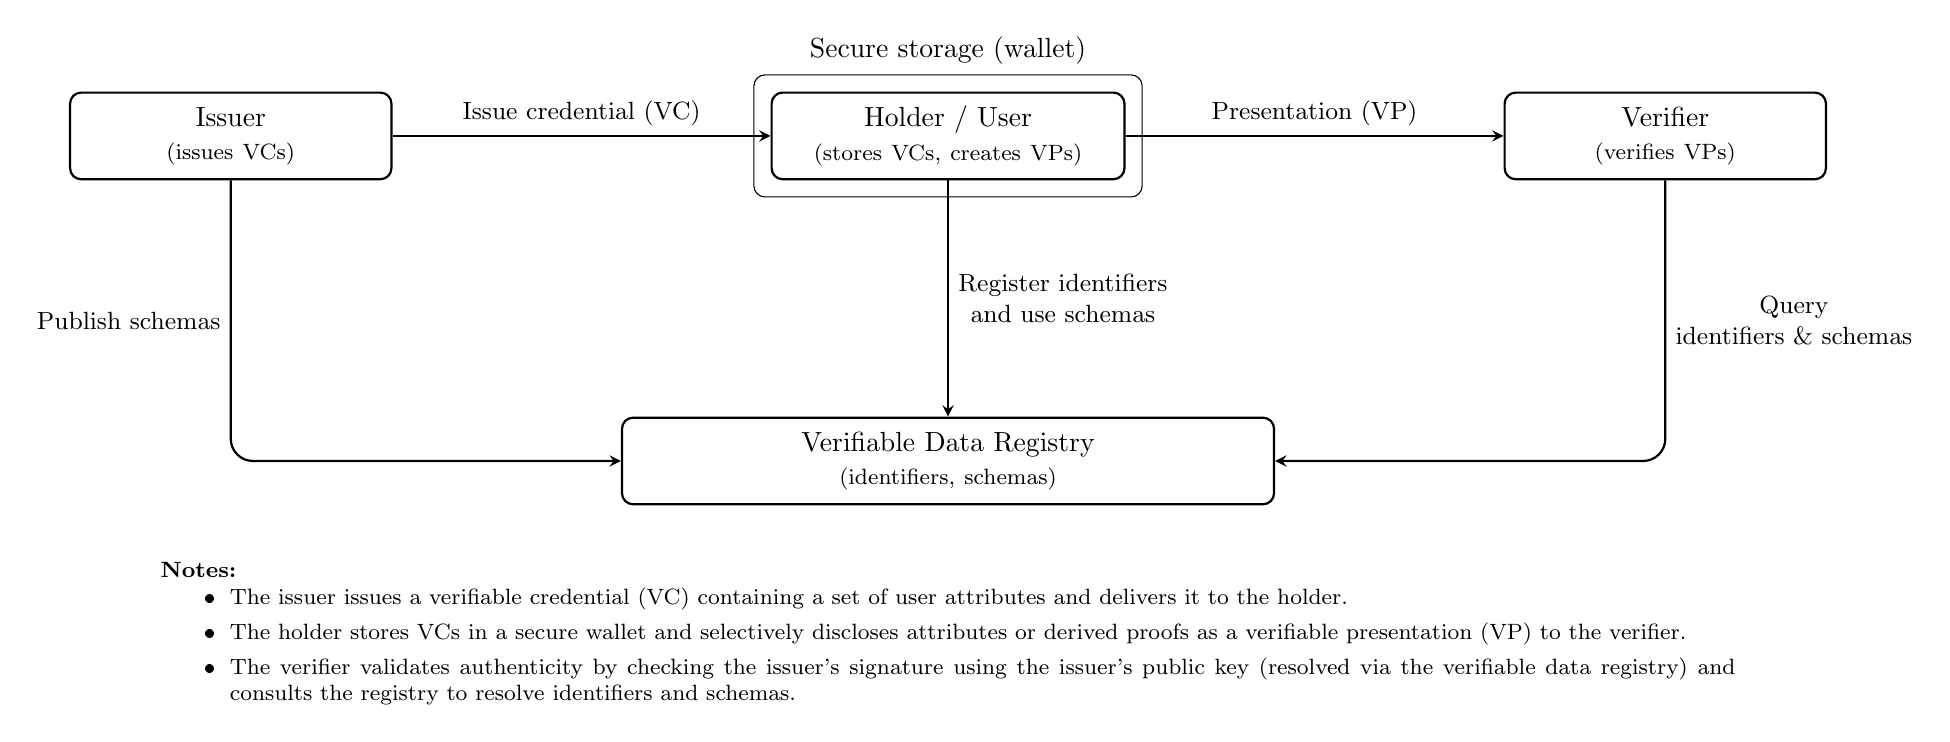
\begin{tikzpicture}[
    entity/.style = {
      draw, thick, rounded corners,
      minimum height=1.1cm,
      align=center,
      inner sep=4pt,
      fill=white
    },
    edge/.style      = {->, >=stealth, thick, rounded corners=8pt},
    smalltext/.style = {font=\small, align=center}
  ]

    \node[entity, text width=3.8cm] (issuer)
      {Issuer\\\footnotesize(issues VCs)};
    \node[entity, right=4.8cm of issuer, text width=4.2cm] (holder)
      {Holder / User\\\footnotesize(stores VCs, creates VPs)};
    \node[entity, right=4.8cm of holder, text width=3.8cm] (verifier)
      {Verifier\\\footnotesize(verifies VPs)};

    \node[draw=black, rounded corners, inner sep=6pt,
          fit=(holder),
          label=above:Secure storage (wallet)] {};

    \node[entity, below=3.0cm of holder, text width=8.0cm] (registry)
      {Verifiable Data Registry\\
       \footnotesize(identifiers, schemas)};

    \draw[edge]
      (issuer.east) --
      node[pos=0.5, above, smalltext] {Issue credential (VC)}
      (holder.west);

    \draw[edge]
      (holder.east) --
      node[pos=0.5, above, smalltext] {Presentation (VP)}
      (verifier.west);

    \draw[edge]
      (issuer.south) |- 
      node[pos=0.25, left, smalltext]
        {Publish schemas}
      (registry.west);

    \draw[edge]
      (holder.south) --
      node[midway, right, smalltext]
        {Register identifiers\\and use schemas}
      (registry.north);

    \draw[edge]
      (verifier.south) |- 
      node[pos=0.25, right, smalltext]
        {Query\\identifiers \& schemas}
      (registry.east);

    % Notes
    \node[align=left, font=\footnotesize, below=0.6cm of registry] {
      \textbf{Notes:}\\
      \begin{minipage}{20cm}
        \vspace{1mm}
        \begin{itemize}\itemsep1pt
          \item The issuer issues a verifiable credential (VC) containing a set of user attributes and delivers it to the holder.
          \item The holder stores VCs in a secure wallet and selectively discloses attributes or derived proofs as a verifiable presentation (VP) to the verifier.
          \item The verifier validates authenticity by checking the issuer's signature using the issuer's public key (resolved via the verifiable data registry) and consults the registry to resolve identifiers and schemas.
        \end{itemize}
      \end{minipage}
    };

  \end{tikzpicture}%
  }
  \caption{Digital identity system}
  \label{fig:did_sys}
\end{figure}


Examples of such digital identity frameworks and credential formats that can be potentially compatible with OpenAC include:
\begin{itemize}
  \item \textbf{eIDAS / EUDI Architecture and Reference Framework} -European digital identity systems in which 
  qualified trust service providers or public authorities issue digitally signed identity 
  attributes that citizens can present via the EUDI Wallet.

  \item \textbf{Mobile Driver’s Licenses (mDL, ISO~18013-5)} - Government agencies issue a 
  digitally signed set of driving-related attributes (e.g., name, age, license class), which 
  users present to relying parties such as law enforcement or age-restricted service providers.

  \item \textbf{Verifiable Credentials (W3C VCDM)} -A general-purpose model where an issuer 
  signs JSON-LD or SD-JWT-based claims about a subject; holders store these credentials and 
  present them to verifiers who validate the issuer’s signature.

  % \item \textbf{Bank-Issued Digital Identity Schemes} --- Financial institutions validate 
  % customer identity information (e.g., KYC data) and issue signed digital credentials that can 
  % be reused for onboarding in other financial or commercial services.

  % \item \textbf{University or Organizational ID Systems} --- Institutions issue digitally 
  % signed attestations (e.g., enrollment status, roles, or qualifications) that students or 
  % employees can present to external verifiers for access to services or discounts.

  % \item \textbf{National Digital ID Cards (e.g., Estonia eID)} --- Government-issued smartcards 
  % or mobile IDs contain signed identity attributes that citizens present for authentication and 
  % authorization in public and private sector services.
\end{itemize}


%ChatGPT except the footnote and the box

\noindent\textbf{Anonymous Credentials from Existing Digital Identity.} We focus on constructing anonymous credentials for 
\emph{existing} digital identity systems without requiring changes to the current issuance flow whilst 
enabling selectively disclosed presentations in an unlinkable manner. 

A central target of this work is the \emph{EUDI ARF}, which specifies how digital identities and credentials are issued, stored, and presented within the EUDI ARF.
While our terminology in this section follows the generic issuer–holder–verifier model, Section~\ref{subsec:aligneudi} restates the same roles using the Wallet User, Relying Party, and EAA vocabulary of the EUDI ARF.
Our construction is designed to integrate with this framework in a modular  manner, allowing anonymous credentials to be derived from standard verifiable credentials, 
whilst complying with its security, interoperability, and regulatory requirements.\footnote{The EU Digital Identity Wallet will be launched in all member states by the end of 2026, with strong requirements for unlinkability with respect to relying parties and identity providers.
According to the Cryptographers' Feedback on the EU Digital Identity’s ARF\footnote{\url{https://github.com/user-attachments/files/15904122/cryptographers-feedback.pdf}}, an Anonymous Credential AC scheme is a suitable cryptographic primitive to instantiate the new EU Digital Identity Wallet (EUDIW, ARF version 1.4.0~\cite{EU:EUDI24}), which is an important step towards developing interoperable digital identities in Europe for the public and private sectors.}

\begin{framed}\footnotesize
	Informally speaking, an \emph{Anonymous Credential} AC scheme allows:
	\begin{itemize}
		\item An \emph{Identity Provider} or \emph{Issuer} IP to (possibly blindly\footnote{i.e. the IP does not know the content that it signs, only its provenance is satisfied.}) sign a set of (eligible) attributes for a \emph{User} U;
		\item The \emph{User} U can show, only if they hold the signed attributes (a.k.a \emph{Unforgeability}), usually through a \emph{Presentation}, to a \emph{Relying Party} RP such that:
		\begin{itemize}
			\item The RP can verify that the set of attributes (signed by IP) that the User U holds satisfy some condition of their interest (a.k.a Correctness);
			\item The RP cannot learn any \emph{additional}\footnote{We stress that the RP may have obtained some privacy sensitive information prior to this presentation.} information beyond the fact that the condition is satisfied or information that can be inferred from the satisfaction of the condition (a.k.a Zero-Knowledge or Anonymity);
			\item The immediate previous requirement also implies that the RP cannot link the various presentations by the same User U (a.k.a. Unlinkability);
		\end{itemize}
		\item The IP can revoke all or a part of the signed attributes that it has issued to the User U, from upon which, the eligible attributes of the User U are updated, and subsequent presentations have to be based on the new and updated attributes (a.k.a \emph{Revocation});
		\item The User U cannot transfer its set of signed attributes to another User U' (a.k.a \emph{Non-transferability}).
	\end{itemize}
\end{framed}

\noindent\textbf{A Generic AC Framework.} In a generic AC framework, the \emph{Issuer} is an entity that uses a fixed public-key 
algorithm (e.g., RSA or ECDSA) and verifiable credential format (such as SD-JWT or mDL) to assert claims about one or more subjects. Since issuer elements are 
typically difficult to modify once deployed, the proposed change are to the holder’s 
wallet and to the relying party (verifier).

The wallet operates in two phases. 
During an offline \emph{Prepare} phase, run once per credential, the wallet:
 \begin{enumerate}
    \item Verifies the Issuer’s signature using standard libraries
    \item Parses and normalizes credential attributes (e.g., converting a 
date of birth to an integer age)
    \item Commits to the attributes using a binding and hiding commitment scheme. 
\end{enumerate}
During the online \emph{Show} phase, which is run for each presentation, the wallet:
\begin{enumerate}
\item Selects the attributes or predicates required by the \emph{Relying Party}
\item Prove them in zero knowledge against the stored commitments
\item Adds a fresh device signature over the session challenge to ensure device binding.
\end{enumerate}

Noticeably, a key requirement of our framework is \emph{modularity}: issuer-signature verification, attribute commitment, predicate proofs, and device binding are defined as separate modules with clear interfaces.
This separation allows the underlying proof system to be replaced for quantum-proofing without modifying other components. 


%ChatGPT, some mods
\medskip
\noindent\textbf{Related Work and Our Proposal.} There exists several prominent approaches to constructing anonymous credentials 
from existing digital identity systems, including the BBS$+$ proposal~\cite{SCN:AuSusMu06,EPRINT:CamDriLeh16}, Microsoft’s \emph{Crescent}~\cite{cryptoeprint:2024/2013}, and Google’s \emph{Longfellow}~\cite{cryptoeprint:2024/2010}. 
Although each of these schemes enables some form of unlinkable selective disclosure, they exhibit limitations in practicality or generality that our design aims to overcome.

The BBS$+$ approach requires modifications to the issuer’s existing credential-issuance flow, 
thereby reducing compatibility with established digital identity infrastructures. The Crescent system 
relies on a trusted setup, which introduces transparency concerns and operational overhead for 
ecosystem deployment. The Longfellow construction, while efficient, is tailored specifically to 
ECDSA-based identity systems and thus lacks general applicability across heterogeneous credential formats.

Our proposal offers an \emph{open} and \emph{fully transparent} design that imposes 
no changes on the issuer workflow, supports modular ``plug-and-play’’ integration with diverse 
credential systems, and requires no trusted setup. Furthermore, our proof-of-concept implementation 
demonstrates best-in-class proving performance, including efficient execution on mobile devices, 
which is essential for real-world usability in frameworks such as the EUDI Wallet.

%Below is by YT
A summary of the existing solutions and our proposal with respect to the AC Framework is presented in Table~\ref{tab:rw-snapshot}. We additionally adapt a comparison for a 1920-byte credential from Vega~\cite{kaviani2025vega}, a concurrent work that follows the similar prepare-and-prove paradigm.\footnote{We have not yet attempted to compare our work with Vega in this version, we will conduct a more detailed analysis of Vega in the next version.}
For OpenAC, the four latency columns follow the same convention as Vega: \emph{Setup} covers the proof system setup for the Prepare and Show circuits; \emph{Precomp.} is the one-time offline Prepare work; \emph{Prove} is the online Show work for a single presentation; and \emph{Verify} is the verifier’s work across both phases.
The proof size column reports the sum of the Prepare and Show proof sizes, and the PK/VK columns give the total proving and verifying key sizes for the two circuits.

We consider a client–server setting with a mobile prover and a server-side verifier.
The verifying key, which is dominated by the Prepare circuit, is large but kept in memory on the verifier side and reused across many proof verifications, while the prover runs under tighter latency and resource constraints.
For consistency with Vega, Table~\ref{tab:openac-main} reports measurements on commodity desktop hardware; mobile measurements and a more detailed benchmarking discussion, including a breakdown from the wallet’s perspective, appear in Section~\ref{sec:benchmarks}.

\begin{table}[h]
\centering
\label{tab:rw-snapshot}
\caption{Comparison of related approaches.}
\footnotesize
\begin{tabularx}{\linewidth}{
  @{}
  >{\RaggedRight\arraybackslash}p{0.17\linewidth}  
  >{\RaggedRight\arraybackslash}p{0.14\linewidth}  
  >{\RaggedRight\arraybackslash}p{0.16\linewidth}  
  >{\RaggedRight\arraybackslash}p{0.21\linewidth}  
  >{\RaggedRight\arraybackslash}p{0.19\linewidth}  
  @{}
}
\toprule
\textbf{Feature} & \textbf{BBS/BBS+} & \textbf{Longfellow} & \textbf{Crescent} & \textbf{OpenAC} \\
\midrule
Issuer modification & Required & None & None & None \\
\addlinespace[0.3em]
Offline phase       & None & None & Lightweight, reusable Prepare & Lightweight, reusable Prepare \\
\addlinespace[0.3em]
Setup               & Pairing-based (no trusted setup) & Transparent & Large, per-circuit trusted setup & Transparent \\
\addlinespace[0.3em]
Proof mechanism     & Pairing-based signatures + ZK proofs & Sum-check + Ligero; custom ECDSA/SHA-256 circuits & Groth16 + Pedersen vector commitments; re-randomizable artifacts & Sum-check; Hyrax-style vector commitments \\
\addlinespace[0.3em]
Device binding      & Optional & Included & Optional & Integrated (in-circuit) \\
\addlinespace[0.3em]
Reusability         & No & No & Yes & Yes \\
\bottomrule
\end{tabularx}

\end{table}

% \begin{table}[h!]
% \centering
% \renewcommand{\arraystretch}{1.2}
% \setlength{\tabcolsep}{6pt}

% \begin{tabular}{l|cccc|ccc|>{\centering\arraybackslash}p{1.3cm}} 
% \hline
% \multirow{2}{*}{\textbf{Scheme}} &
% \multicolumn{4}{c|}{\textbf{Latency (ms)}} &
% \multicolumn{3}{c|}{\textbf{Size (kB)}} &
% \multirow{2}{*}{\textbf{\shortstack{Trans.\\Setup}}} \\  
% & \textit{Setup} & \textit{Precompute} & \textit{Prove} & \textit{Verify} &
%   \textit{Proof} & \textit{pk} & \textit{vk} \\
% \hline
% Longfellow & 7235 & ---    & 680 & 324 & 325 & 202     & 202   & \checkmark \\
% Crescent   & 172\,437 & 14\,725 & 237 & 118 & 16 & 710\,565 & 1 & $\times$ \\
% Vega\textsubscript{SC} & 3689 & 238 & 247 & 55 & 99 & 6562  & 6561 & \checkmark \\
% Vega\textsubscript{MC} & 193  & 109 & 212 & 51 & 150 & 436   & 436  & \checkmark \\
% OpenAC  &  5230   & 3016    &     &     &     &      &      & \checkmark \\
% \hline
% \end{tabular}

% \caption{Performance comparison for a 1920-byte MSO (latency in ms, sizes in kB), adapted from Vega~\cite{kaviani2025vega}}
% \label{tab:rw-perfcomp}
% \end{table}


\begin{table}[t]
\centering
\caption{Performance comparison for a 1920-byte MSO, adapted from Vega~\cite{kaviani2025vega}.}
\scriptsize
\setlength{\tabcolsep}{3pt}
\renewcommand{\arraystretch}{1.1}
\begin{tabular}{l|cccc|ccc|c} 
\hline
\multirow{2}{*}{\textbf{Scheme}} &
\multicolumn{4}{c|}{\textbf{Latency (ms)}} &
\multicolumn{3}{c|}{\textbf{Size (kB)}} &
\multirow{2}{*}{\textbf{\shortstack{Trans.\\Setup}}} \\ 
& \textit{Setup} & \textit{Precomp.} & \textit{Prove} & \textit{Verify} &
  \textit{Proof} & \textit{pk} & \textit{vk} \\
\hline
Longfellow      & 7\,235   & ---    & 680 & 324 & 325 & 202     & 202   & \checkmark \\
Crescent        & 172\,437 & 14\,725 & 237 & 118 & 16  & 710\,565 & 1   & $\times$ \\
Vega\textsubscript{SC} & 3\,689   & 238    & 247 & 55  & 99  & 6\,562  & 6\,561 & \checkmark \\
Vega\textsubscript{MC} & 193     & 109    & 212 & 51  & 150 & 436     & 436   & \checkmark \\
\hline
OpenAC & 
4193 &    % Setup (Prepare + Show setup) 4157 + 36
3442 &    % Precomp (Prepare Prove + Reblind Prepare) 2727 + 715
102 &     % Prove (Show Prove + Reblind Show) 77 + 25
83 &    % Verify (Prepare Verify + Show Verify) 74 + 9
149.7 &   % Proof size (Prepare proof + Show proof) 109.29 + 40.41
433664 &  % Proving key size: Prepare Proving Key + Show Proving Key 420.05MB + 3.45MB
433664 &  % Verifying key size: Prepare Verifing Key + Show Verifying Key
\checkmark \\
\hline
\end{tabular}
\vspace*{0.3cm}
\begin{minipage}[t]{0.8\textwidth}
    The Longfellow, Crescent, and Vega benchmarks are done in Azure Standard\_F16as\_v6 VM with 16 vCPUs and 64 GB RAM while we consider a commodity hardware (MacBook Pro, M4, 14-core GPU, 24GB RAM).
\end{minipage}
\label{tab:openac-main}
\end{table}



% In the aforementioned feedback document, BBS~\cite{C:BonBoySha04, C:CamLys04} and BBS+~\cite{SCN:AuSusMu06,EPRINT:CamDriLeh16}
% %\footnote{For BBS, thanks to prior work by the W3C, the Decentralized Identity Foundation, IETF/IRTF, ISO, and other standardization bodies, as well as the availability of open-source software libraries, the EC can develop a standard and reference implementation with only a modest effort. The feedback additionally recommend that the EUDI be designed following the principle of crypto-agility, meaning that its underlying technologies can be upgraded quickly in the future if the need arises.} 
% were promoted as the main candidate, besides that, there have been two independent works from Google~\cite{cryptoeprint:2024/2010} (longfellow) and Microsoft~\cite{cryptoeprint:2024/2013} (Crescent) that attempted to offer candidate solutions. In this document, we attempt to offer a new candidate, called \textbf{zkID}.

% In comparison, these approaches show the current trade-off: systems either reuse existing issuer infrastructure but pay high per-presentation costs, or they achieve fast online proofs at the price of large setups and pairing-based assumptions. 
% \begin{quote}
% 	\emph{The zkID construction aims to combine issuer compatibility with reusable offline work, while remaining transparent and modular.}
% \end{quote}

% \paragraph{Organization}
% The remainder of this document is organized as follows: Section~\ref{sec:appeudi} introduces the EUDI setting and maps its requirements to our construction, Section~\ref{sec:preliminaries} introduces the notation and cryptographic tools, Section~\ref{sec:contribution} describes the technical details of our zkID construction, Section~\ref{sec:security} provides the security analysis and proofs, Section~\ref{sec:benchmarks} reports benchmark results, and Section~\ref{sec:conclusion} concludes.

% \subsection{Our zkID}
% We work with SD--JWT credentials, extensions to other formats are straightforward. The construction adds a zero-knowledge layer around the issued credential and is instantiated with Spartan as the proof system and Hyrax-style Pedersen vector commitments; standard zero-knowledge blinding is applied.

% \paragraph{Objects and notation.}
% Let $S$ be the issued credential with messages $(m_1,\dots,m_N)$, per-message salts $(s_1,\dots,s_N)$, hashes $(h_1,\dots,h_N)$, and issuer signature $\sigma_I$ under public key $PK_I$. The wallet public key $PK_W$ is included among the messages. A presentation policy is modeled as predicates $f_1,\dots,f_K$ over $(m_i)$.

% \paragraph{Two relations.}
% Proving is split into two relations with a fixed interface:
% \begin{itemize}[leftmargin=1.2em]
%   \item Prepare: Once per credential, prove the correct parsing of $S$, that $h_i=\mathrm{SHA256}(m_i,s_i)$ for all $i$, that $\mathrm{Verify}(\sigma_I,PK_I)=1$, and compute a Hyrax commitment $C_m$ to the \emph{message vector} $(m_i)$. This relation is independent of the presentation policy; its proof can be re-randomized and reused.
%   \item Show: For a given policy, prove that each requested predicate $f_j(m_1,\dots,m_N)$ holds and that a live signature on the verifier’s challenge verifies under the wallet public key bound in $S$. Publish a commitment $C'_m$ to the same message vector.
% \end{itemize}
% The link is enforced by checking $C_m=C'_m$ (Hyrax commitment equality), so no auxiliary link primitive is required. Because equality is checked in one group, both relations use the same curve.

% \paragraph{Workflow.}
% Issuance produces $S$ and binds it to $PK_W$. At presentation, the verifier sends a fresh challenge $\mathsf{nonce}_V$; the wallet signs $\mathsf{nonce}_V$ with the corresponding secret key and returns $(\pi_{\texttt{prepare}},\pi_{\texttt{show}})$. The verifier validates both proofs and accepts only if $C_m=C'_m$.

% \subsection{Comparison to alternatives}\label{subsec:comparison}

% \paragraph{Setting the AC Framework.}
% Let us first outline a reference architecture that represents what an anonymous-credential system would ideally look like if it is to integrate smoothly with current infrastructures. 
% In this model, the \emph{Issuer} is treated as a fixed component that continues to use its existing public-key algorithms (such as RSA or ECDSA) and standard credential formats (e.g., JWT or mDL), since it's typically difficult to change once deployed. All additional logic is placed in the user’s wallet and the verifier.

% The wallet is expected to operate in two stages: an offline \emph{Prepare} step, which verifies the Issuer’s signature once using standard libraries, parses and normalizes credential attributes (for example, turning a date of birth into an integer age), and commits to those attributes using a binding and hiding commitment scheme (a cryptographic way to lock values so they can later be revealed or proven in restricted form); and an online \emph{Show} step, which runs per presentation, where the wallet selects only the attributes or predicates required by a \emph{Relying Party}’s policy, proves them in zero knowledge against the stored commitments, and includes a fresh device signature over the session challenge to ensure the proof is tied to the holder’s device.

% A further requirement is \emph{modularity}: each major function, issuer signature verification, attribute commitment, predicate proofs, and device binding, should be defined as a separate module with a clear interface. This separation makes it possible to swap the underlying proof engine (for example, using a SNARK today or a post-quantum proof system in the future) without requiring changes to parts of the system that are costly or impractical to modify. The purpose of this modular view is to act as a comparison framework: it outlines how a deployment-friendly anonymous-credential stack could be structured, making it easier to compare proposals by the modules they cover, the constraints they address, and the trade-offs they make. 

% A summary of them with respect to the AC Framework is presented in Table~\ref{tab:rw-snapshot}.

% \paragraph{BBS-based anonymous credentials.~\cite{baum2024cryptographers}}
% BBS-based anonymous credentials are recommended in public feedback for the EUDI wallet as a way to meet the program’s requirement that presentations must not be tracked, linked, or correlated~\cite{baum2024cryptographers}.
% This work treats a credential as a constant-size signature on a vector of attributes in pairing-friendly groups, as introduced by Boneh–Boyen–Shacham and proven secure for BBS+ by Au–Susilo–Mu~\cite{C:BonBoySha04,SCN:AuSusMu06}.
% A holder then produces zero-knowledge proofs that reveal only the required attributes or predicates; each presentation is freshly generated so separate verifications cannot be linked.
% This matches our reference system view on the presentation side-privacy enforced at the holder with per-session, non-repeating outputs.
% Where these designs differ from our constraints is issuance. To use BBS/BBS+, issuers sign credentials with a pairing-based scheme rather than the RSA or ECDSA schemes used today~\cite{C:BonBoySha04,SCN:AuSusMu06}. To remain compatible with standardized curves such as P-256 while keeping public verifiability, a pairing-free, server-aided variant (often termed BBS\#) allows the holder to prefetch small auxiliary data through an oblivious interaction with an issuer-side helper and later perform non-interactive presentations; the helper data scales linearly with the number of planned presentations~\cite{cryptoeprint:2025/513}.
% In both variants, device binding and revocation checks can be encoded as attributes or verified within the proof so that transcripts and status queries avoid stable identifiers.


% \paragraph{Anonymous Credentials from ECDSA.~\cite{cryptoeprint:2024/2010}}
% This work considers environments where credential issuers already sign with ECDSA on standardized curves (such as P-256) and hash data with SHA-256.
% The main challenge is that proving correctness of an ECDSA signature in zero knowledge is costly with standard proof systems, because the arithmetic used in P-256 and the bit-level operations in SHA-256 do not align well with the fast polynomial techniques (such as number-theoretic transforms, a method that speeds up polynomial multiplication over special fields) that many modern ZK libraries rely on.
% To handle this, the authors introduce custom circuits for ECDSA and SHA-256, and use a layered protocol based on the sum-check technique with a lightweight encoding (Reed–Solomon code) to control proof size.
% An additional “consistency check” ensures that the same hidden signing key is used across both the signature and the hash logic.
% At presentation, the wallet produces a proof for the verifier and the device also signs a fresh challenge (this is the device-binding step: a live signature that ties the proof to the holder’s device).
% In terms of the reference system view, issuer compatibility is preserved, selective disclosure is supported, and device binding is included; however, there is no reusable offline phase, so the full proof is generated at every presentation. The reported costs are about 60\,ms to prove one ECDSA signature and about 1.2\,s for a complete mDL presentation on mobile devices~\cite[\S5.3,\S6.2]{cryptoeprint:2024/2010}, with larger proof sizes and higher verifier effort than systems based on succinct setup-dependent SNARKs.

% \paragraph{Crescent Credentials.~\cite{cryptoeprint:2024/2013}}
% This work considers environments where issuers continue using existing credential formats such as JWT or mDL and their current signing keys, so no issuer-side changes are required.
% Its workflow is split into a heavy one-time Prepare phase and a lightweight per-presentation Show phase.
% In Prepare, the wallet verifies the issuer’s signature, parses the credential into attributes, and creates two reusable artifacts, that is, cryptographic objects the wallet reuses across presentations: (i) a Groth16 proof that these checks were done correctly, and (ii) a Pedersen vector commitment over the attributes, enabling selective disclosure.
% Both artifacts support re-randomization for unlinkability.
% In the Show phase, the wallet re-randomizes the prepared artifacts and attaches only the proofs required by the verifier’s policy, such as proving an age threshold or linking two credentials to the same holder. Device binding can be added at this step by letting the secure element sign the verifier’s challenge.
% In terms of the reference system view, Crescent realizes the two-phase design with reusable offline work and modular predicates, while leaving issuers unchanged. The trade-offs are significant: the Prepare phase is heavy (tens of seconds for JWTs and minutes for mDLs), the scheme depends on pairing-based Groth16 proofs with a large trusted setup ($\approx$ 661 MB-1.1 GB~\cite[\S4]{cryptoeprint:2024/2013}), and the security model is classical only, without post-quantum protection. The Show step, however, runs with low latency-typically 22-41\,ms with $\approx$1 KB proofs, or about 315\,ms with device binding~\cite[\S4]{cryptoeprint:2024/2013}.

% \begin{table}[t]
% \centering
% \caption{Comparison of related approaches.}
% \label{tab:rw-snapshot}
% \footnotesize
% \begin{tabularx}{\linewidth}{l >{\RaggedRight\arraybackslash}X >{\RaggedRight\arraybackslash}X >{\RaggedRight\arraybackslash}X >{\RaggedRight\arraybackslash}X}
% \toprule
% \textbf{Feature} & \textbf{BBS/BBS+} & \textbf{AC from ECDSA} & \textbf{Crescent} & \textbf{zkID (ours)} \\
% \midrule
% Issuer modification & Required & None & None & None \\
% Offline phase       & None & None & Heavy Prepare; light Show & Lightweight, reusable Prepare \\
% Setup               & Pairing-based (no trusted setup) & Transparent & Large, per-circuit trusted setup & Transparent \\
% Proof mechanism     & Pairing-based signatures with ZK proofs & Sum-check with Ligero; custom ECDSA/SHA-256 circuits & Groth16 with Pedersen vector commitments; re-randomizable artifacts & Transparent sum-check; Hyrax-style vector commitments \\
% Device binding      & Optional & Included & Optional & Integrated (in-circuit) \\
% Reusability         & No & No & Yes & Yes \\
% \bottomrule
% \end{tabularx}
% \end{table}


% \subsection{Our zkID}

% \kwnote{A table or figure that summarizes the pros and cons of other approaches and ours will be very helpful for readers.}

% Our construction works with standardized credentials (e.g., SD-JWT, mDL) and existing PKI (RSA/ECDSA), so issuers do not need to change their issuance pipelines.
% The zkID workflow follows the two-phase split in the reference view: a one-time Prepare phase and a per-presentation Show phase.
% In Prepare, the wallet verifies the issuer’s signature, parses the credential into normalized messages, computes the associated hashes, and produces two reusable artifacts: (i) zero-knowledge proofs that issuer-side checks and parsing were done correctly, and (ii) Hyrax-style Pedersen vector commitments to a designated message column, supporting efficient proofs over multiple attributes.
% In Show, the wallet proves only the verifier’s requested predicates and includes a fresh device-binding signature. To link Prepare and Show without revealing values, the verifier checks equality of commitments across both proofs; the wallet reuses the corresponding randomness for that session.
% The proving backend is transparent (no trusted setup). It checks the arithmetic constraints with a sum-check–style protocol and uses a small inner-product check to verify commitment openings. For device binding, we choose a curve whose scalar field matches the device’s signature field (e.g., P-256), so the device signature can be verified directly inside the proof without emulation or field translation. 
% In terms of the reference system view, issuer compatibility is preserved, the two-phase reuse is integrated into the workflow, predicates are modular, and there is no trusted setup. The trade-offs are that security currently relies on discrete-log assumptions (not post-quantum) and that commitment equality requires using the same curve across Prepare and Show; the modular interface leaves room to swap in lattice-based commitments when suitable.

\section{Technical Overview and Applicability to EUDI ARF}
\label{sec:appeudi}

% \noindent\textbf{OpenACTAL.} We work with SD--JWT credentials; extensions to other formats are straightforward. The construction adds a zero-knowledge layer around the issued credential and is instantiated with Spartan as the proof system and Hyrax-style Pedersen vector commitments; standard zero-knowledge blinding is applied.

% Let $S$ be the issued credential with messages $(m_1,\dots,m_N)$, per-message salts $(s_1,\dots,s_N)$, hashes $(h_1,\dots,h_N)$, and issuer signature $\sigma_I$ under public key $PK_I$. The wallet public key $PK_W$ is included among the messages. A presentation policy is modeled as predicates $f_1,\dots,f_K$ over $(m_i)$. Proving is split into two relations with a fixed interface:
% \begin{itemize}[leftmargin=1.2em]
%   \item Prepare: Once per credential, prove the correct parsing of $S$, that $h_i=\mathrm{SHA256}(m_i,s_i)$ for all $i$, that $\mathrm{Verify}(\sigma_I,PK_I)=1$, and compute a Hyrax commitment $C_m$ to the \emph{message vector} $(m_i)$. This relation is independent of the presentation policy; its proof can be re-randomized and reused.
%   \item Show: For a given policy, prove that each requested predicate $f_j(m_1,\dots,m_N)$ holds and that a live signature on the verifier’s challenge verifies under the wallet public key bound in $S$. Publish a commitment $C'_m$ to the same message vector.
% \end{itemize}
% The link is enforced by checking $C_m=C'_m$ (Hyrax commitment equality), so no auxiliary link primitive is required. Because equality is checked in one group, both relations use the same curve.

% Issuance produces $S$ and binds it to $PK_W$. At presentation, the verifier sends a fresh challenge $\mathsf{nonce}_V$; the wallet signs $\mathsf{nonce}_V$ with the corresponding secret key and returns $(\pi_{\texttt{prepare}},\pi_{\texttt{show}})$. The verifier validates both proofs and accepts only if $C_m=C'_m$.

% Let $S$ be an issued credential containing messages $(m_1,\dots,m_N)$, per-message salts 
% $(s_1,\dots,s_N)$, hashes $(h_1,\dots,h_N)$, and an issuer signature $\sigma_I$ under public key 
% $PK_I$. The wallet public key $PK_W$ is included among the messages. A presentation policy is 
% modeled as predicates $f_1,\dots,f_K$ over the message vector. Proving is divided into two relations 
% with a fixed interface:
% \begin{itemize}[leftmargin=1.2em]
%   \item \textbf{Prepare:} Once per credential, prove that $S$ is parsed correctly, that 
%   $h_i=\mathrm{SHA256}(m_i,s_i)$ for all $i$, and that $\mathrm{Verify}(\sigma_I,PK_I)=1$. Compute a 
%   Hyrax commitment $C_m$ to the message vector $(m_i)$. This relation is policy-independent; its 
%   proof can be re-randomized and reused.
%   \item \textbf{Show:} For a given policy, prove that each requested predicate 
%   $f_j(m_1,\dots,m_N)$ holds and that a live signature on the verifier’s challenge verifies under 
%   the wallet public key bound in $S$. Publish a commitment $C'_m$ to the same message vector.
% \end{itemize}

% The two phases are linked by checking $C_m = C'_m$ (Hyrax commitment equality), eliminating the need 
% for auxiliary link primitives. Because equality is checked in a single group, both relations operate 
% on the same curve.

% Issuance produces $S$ and binds it to $PK_W$. During presentation, the verifier sends a fresh 
% challenge $\mathsf{nonce}_V$; the wallet signs $\mathsf{nonce}_V$ with the corresponding secret key 
% and returns $(\pi_{\texttt{prepare}},\pi_{\texttt{show}})$. The verifier validates both proofs and 
% accepts only if $C_m = C'_m$.
\subsection{Technical Overview}
\label{subsec:preliminaries}
% \ndhy{This section is a work in progress. It will be completed in the next few days.}
% \paragraph{Notation.}
% For $n\in\mathbb{N}$, let $[n]=\{1,\dots,n\}$.
% Vectors are in bold, e.g., $\mathbf{a}=(a_1,\ldots,a_\ell)$.
% Concatenation is $\|$.
% For a (possibly randomized) algorithm $\mathsf{Alg}$, we write $y \leftarrow \mathsf{Alg}(x)$ for its output.
% The security parameter is $\lambda$, and $\mathrm{negl}(\lambda)$ denotes a negligible function.
% \subsection{Algebraic setting and basic primitives}
% \label{subsec:algebra}
% Let $\mathbb{F}$ be a prime field of order $q$ and $\mathbb{G}$ a cyclic group of order $q$ with generator $g$, where discrete logarithms are hard.
% We use SHA\mbox{-}256 as $\mathsf{H}:\{0,1\}^\ast\!\rightarrow\!\{0,1\}^{256}$.
% The issuer uses a digital signature scheme $\mathsf{Sig}_I=(\mathsf{KeyGen}_I,\mathsf{Sign}_I,\mathsf{Verify}_I)$ (e.g., ECDSA/RSA), and the device uses $\mathsf{Sig}_D$ for nonce-bound session signatures; both are assumed EUF\mbox{-}CMA.

% \paragraph{Pedersen vector commitments.}
% Fix generators $\mathbf{g}=(g_1,\ldots,g_\ell)$ and $h$ in $\mathbb{G}$.
% For $\mathbf{a}\in\mathbb{F}^\ell$ and $r\in\mathbb{F}$ define
% \[
% \mathsf{Com}(\mathbf{a};r)=\prod_{i=1}^{\ell} g_i^{a_i}\cdot h^{r}\in\mathbb{G}.
% \]
% $\mathsf{Com}$ is perfectly hiding and binding under discrete\mbox{-}log hardness.
% We will need efficient \emph{openings} and \emph{equality proofs} for Pedersen commitments; we realize these via inner-product arguments (IPAs) in the Hyrax framework~\cite{SP:WTSTW18}.

% \paragraph{Hyrax commitments.}
% Hyrax commitments \cite{SP:WTSTW18} allow us to commit to a multilinear extension $\widetilde{P}$ of a function $P:\{0,1\}^{\log n} \rightarrow \mathbb{F}$. 
% Notably, we can express $\widetilde{P}(x_1, \dots, x_{\log n})$ as a vector-matrix-vector product $\vec{v_L} P \vec{v_R}$, where:
% \begin{itemize}
%     \item $P$ is a square matrix of evaluations of $P$ on the $\{0,1\}^{\log n}$ hypercube, represented as $\langle \vec{p_i}\rangle_{i \in \sqrt{n}}$ where $\vec{p_i} \in \mathbb{F}^{\sqrt{n}}$ are columns of $P$
%     \item $\vec{v_L}(x_1, \dots, x_{(\log n)/2}) = \langle \widetilde{\chi}_{(b_1, \dots, b_{(\log n)/2})}(x_1, \dots, x_{(\log n)/2})\rangle _{(b_1, \dots, b_{(\log n)/2})\in \{0,1\}^{(\log n)/2}}$, and 
%     \item $\vec{v_R}(x_{(\log n)/2+1}, \dots, x_{\log n}) = \langle \widetilde{\chi}_{(b_{(\log n)/2+1}, \dots, b_{\log n})}(x_{(\log n)/2}, \dots, x_{\log n})\rangle_{(b_{(\log n)/2}, \dots, b_{\log n}) \in \{0,1\}^{(\log n)/2}}$,
% \end{itemize}
% and $\widetilde{\chi}_{b_1, \dots, b_m} (x_1, \dots, x_m) = \prod_{i \in [m]} \widetilde{\chi}_{b_i}(x_i)$, where
% $\widetilde{\chi_{b_i}}(x_i)$ is the multilinear extension of the function $\chi_{b_i}(x_i): \{0,1\} \rightarrow \mathbb{F}$ given by $\chi_{b_i}(x_i) = x_ib_i + (1-x_i)(1-b_i)$, which equals $1$ if $x_i = b_i$ and $0$ otherwise.

% Then our Hyrax commitment scheme is given by:
% \begin{itemize}
%     \item $\textbf{Setup}(1^{\lambda}, n) = (g_i)_{i \in [\sqrt n]}$ where $g_i \in \mathbb{G}$ are elements of the elliptic curve group $\mathbb{G}$ over which we compute our Pedersen commitments.
%     \item $\textbf{Commit}_h(pp, P) \rightarrow (c,S)$, where 
%     $c = \{c_i\}_{i \in [\sqrt{n}]}$ and $S = \{S_i\}_{i \in [\sqrt{n}]}$, and
%     $(c_i, S_i) \leftarrow Commit_p(pp, \langle \vec{p_i} \rangle)$
%     where $Commit_p$ is the Pedersen vector commitment scheme.
%     \item $\textbf{Eval}_h(pp, c, r, v, n; P, S)$, where $r$ is the opening point and $v$ is the claimed evaluation of $P(r)$, is given by:
%     \begin{itemize}
%         \item Prover and Verifier compute $\vec{v_L} = \vec{v_L}(r_1, \dots, r_{(\log n)/2})$, $\vec{v_R} = \vec{v_R}(r_{(\log n)/2+1}, \dots, r_{\log n})$, 
%     and $C = \sum_{i \in [\sqrt{n}]} \vec{v_L}_i c_i$ (where addition is over $\mathbb{G}$)
%         \item Prover and Verifier engage in an interactive IPA protocol to prove that $P(r)$ is a dot product of $v_R$ and $C$ 
%     \end{itemize} 
% \end{itemize} 

% \subsection{Zero-knowledge proving interface}
% \label{subsec:zk-interface}
% We use a \emph{transparent} general-purpose SNARK in the Spartan family~\cite{C:Setty20}, instantiated over $\mathbb{F}$ for R1CS instances.
% Algorithms are
% \[
% \mathsf{pp} \leftarrow \mathsf{Setup}(1^\lambda),\quad
% \pi \leftarrow \mathsf{Prove}(\mathsf{pp},x,w),\quad
% b \leftarrow \mathsf{Verify}(\mathsf{pp},x,\pi)\in\{0,1\},
% \]
% where $x$ is public input and $w$ the witness.
% (We reference succinct CRS-based systems such as Groth16~\cite{groth2016size} later only for performance comparisons.)

% \paragraph{R1CS instance.}
% An \textit{R1CS instance} is a tuple $(\mathbb{F}, A, B, C, io, n, m)$, 
% where $io$ denotes the public input and output of the instance, 
% $A, B, C \in \mathbb{F}^{n \times n}$, where $m \geq |io| + 1$
% and there are at most $m$ non-zero entries in each matrix. An instance is said to be \textit{satisfiable}
% if there exists a witness $\vec{w} \in F^{n - |io| - 1}$ such that
% $(A \cdot Z) \circ (B \cdot Z) = (C \cdot Z),$
% where $\vec{Z} = (io, 1, \vec{w})$, and $\circ$ is the Hadamard (entry-wise) product.

% \paragraph{} Throughout the paper, assume that we are dealing with sparse R1CS instances, where $m = O(n)$.

% \paragraph{R1CS as a language} We let the language 
% \[
% R_{\text{R1CS}} = \{ \langle x = (\mathbb{F}, A, B, C, io, n, m): \text{$x$ is satisfiable }\rangle \}.
% \]
% The language $R_{\text{R1CS}}$ is NP-complete.

% \paragraph{} A Spartan zero-knowledge proof is an argument of knowledge for the R1CS language.
% The Prover can prove not only that a given instance $x \in R_{\text{R1CS}}$, but knowledge of the corresponding witness $\vec{w}$.   
% At a high level, this application considers R1CS instances that represent the computational structure of ownership of a valid credential, along with any other desired properties about the credential. 
% Thus a valid argument of knowledge implies knowledge of the underlying credential that has the claimed properties, which is necessary for real-world authentication.

% % \subsection{Relations used by \textsf{zkID}}
% % \label{subsec:relations}
% % Let $\mathsf{Parse}$ be a deterministic parser that extracts $(\mathbf{a},\mathbf{s},\mathbf{h},\sigma_I,\mathsf{meta})$ from a token $\tau$ (attributes, salts, digests, issuer signature, metadata), consistent with the chosen format (SD\mbox{-}JWT/mDL).

% % \paragraph{Prepare relation $\mathcal{R}_{\mathrm{prep}}$.}
% % \dots
% % \paragraph{Show relation $\mathcal{R}_{\mathrm{show}}$.}
% % \dots

% \subsection{High-Level Credential Presentation Flow}\label{sec:high-level-flow}

% The following outlines the high-level protocol for a credential presentation.

% \begin{enumerate}
% \item The Prover receives a signed credential from an Issuer to be stored securely in their wallet, issued to the Wallet Secure Cryptographic Device (WSCD) public key.
% \item At presentation time, the Verifier sends over challenge $\texttt{nonce}_V$ for device-binding verification.
% \item The Prover signs the challenge \texttt{nonce} with the public key $p_U$ controlled by their WSCD and specified in their credential.
% \item The Prover computes two separate but linked zero-knowledge proofs $\pi_{\text{\texttt{prepare}}}, \pi_{\text{\texttt{show}}}$ which together cover the following statements: SD-JWT parsing, verification of the SD-JWT Issuer signature, 
% proper disclosures and/or arbitrary predicates on the disclosures, and device-binding. 
% (i.e.\ checks the \texttt{nonce} signature against their public key); then sends $\pi_{\text{\texttt{prepare}}}, \pi_{\text{\texttt{show}}}$ to the Verifier.
% \item The Verifier verifies $\pi_{\text{\texttt{prepare}}}, \pi_{\text{\texttt{show}}}$ independently, and also verify that they are linked; grants Prover access to some service based on their credential disclosures.
% \end{enumerate}

% \subsection{Security model}
% \label{subsec:security-model}

% In our security model, we assume that the Prover is malicious, and that each Verifier is semi-honest, meaning that if the Prover presents a valid proof that they own a credential with some property, the Verifier will grant access to any services for which the property suffices.


% For security on the Verifier's side, our soundness analysis considers the probability that a Prover without real ownership of a valid credential can generate a false proof of ownership. 


% For security on the Prover's side, we guarantee that our proofs are zero-knowledge, so that a semi-honest computationally bounded Verifier cannot get any additional private information about the Prover's credential given the proof, beyond what is publically revealed in the proof.
% In particular, we do not consider the case where the Verifier is malicious, where e.g. a false Verifier pretends to be an authorized Verifier. The problem of Verifier identity lies outside the scope of this paper.


% Futhermore, we assume that Verifiers can collude, i.e. that Verifiers $V_1, \dots, V_N$ that have receieved proofs $\{\pi_1\}, \dots, \{\pi_N\}$ from a given Prover $P$ can compute functions $f(\pi_1, \dots, \pi_N)$. 
% Therefore, we desire the \textbf{unlinkability property}: given $pi_1, \dots, \pi_N$, the Verifiers should not be able to determine whether or not any two of these proofs came from the same Prover $P$.
% Note that this requires the Prover to re-randomize each presentation's proof; a static zero-knowledge proof of the same statement, while not revealing private credential information, will still look the same.
% It is possible that Verifier's can effectively de-anonymize a Prover by linking their anonymous activity across presentations and analyzing corresponding metadata, e.g. time of presentation.

\paragraph{Notation}
For $n \in \mathbb{N}$, we write $[n]=\{1,\ldots,n\}$. Bold letters denote vectors, e.g., $\mathbf{m}=(m_1,\ldots,m_n)$. Concatenation is written $\|$. The security parameter is $\lambda$; $\mathsf{negl}(\lambda)$ denotes a negligible function. For a (possibly randomized) algorithm $\mathsf{Alg}$, we write $y \leftarrow \mathsf{Alg}(x)$ for its output on input $x$. 

We follow the generic W3C VC roles:
\begin{itemize}
  \item The \emph{issuer} $I$ signs credentials with a long-term key pair $(SK_I,PK_I)$ (e.g., ECDSA P--256 or RSA).
  \item The \emph{prover} $P$ is the holder’s wallet, which stores credentials and generates proofs. 
  \item The \emph{verifier} $V$ is the relying party that checks proofs against a policy.
\end{itemize}
For device binding, the prover’s secure element holds an additional signing key pair $(SK_D,PK_D)$ used only to sign fresh per-session challenges.

\paragraph{Credentials}
A credential is a standardized signed object $S$ (e.g., SD--JWT~\cite{IETF:FetYasCam25} or mDL~\cite{ISO:18013-5}). 
Parsing maps $S$ into an ordered vector of attributes
\[
  \mathbf{m}=(m_1,\ldots,m_n).
\]
Non-numeric fields (strings, dates) are encoded injectively into integers. 
The resulting integers are interpreted in a prime field $\mathbb{F}=\mathbb{F}_q$ chosen for the proof backend. 
For each attribute $m_i$ we sample a salt $s_i \leftarrow \mathbb{F}$ and compute
\[
  h_i = \mathsf{H}(m_i \,\|\, s_i),
\]
where $\mathsf{H}$ is instantiated as SHA--256. 
The issuer’s signature is
\[
  \sigma_I = \mathsf{Sign}_{SK_I}(h_1,\ldots,h_n),
\]
verified under $PK_I$.

\paragraph{zk-SNARKs.}
We summarise the zk-SNARK terminology used in this paper.
A zk-SNARK is a non-interactive proof system between a prover and a verifier in which the prover, holding some private data (the \emph{witness}) and public data (the \emph{public input}), produces a short proof that the public input and witness satisfy a given relation, and the verifier decides whether to accept the proof using only the public input~\cite{EC:Groth16}.
In our setting, the zk-SNARK prover is always in the holder wallet $P$ and the zk-SNARK verifier is always the relying party $V$.

Many zk-SNARK and succinct argument constructions are specified with a setup algorithm that outputs public parameters, typically split into a proving key (used by the prover) and a verifying key (used by the verifier)~\cite{EC:GGPR13,USENIX:BCTV14,EC:Groth16,C:Setty20}.
In pairing-based systems such as Groth16 and related schemes~\cite{EC:GGPR13,USENIX:BCTV14,EC:Groth16}, this setup is usually described in terms of a structured reference string generated using secret randomness; if this randomness were ever revealed, an adversary could in principle construct convincing proofs for false statements.
We refer to this as a \emph{trusted setup}.
In contrast, transparent argument systems such as Spartan derive their public parameters from public randomness or a fixed public description and do not rely on a trapdoor in the setup~\cite{C:Setty20}.

We use standard notions of \emph{correctness}, \emph{soundness}, and \emph{zero-knowledge}~\cite{Goldreich01}.
Correctness means that an honest prover, given a true statement and an appropriate witness, produces proofs that an honest verifier accepts.
Soundness means that no efficient prover can make an honest verifier accept a false statement, except with negligible probability.
Zero-knowledge means that the Verifier learns nothing beyond the validity of the statement; informally, there exists an efficient simulator that can produce indistinguishable proofs without using the witness.
When we refer to a \emph{lightweight} prover, we mean that, although zk-SNARK provers are typically the dominant cost compared to verification~\cite{EC:Groth16}, our prover fits within the latency and memory constraints of the target mobile devices, as shown in Section~\ref{sec:benchmarks}.
In the remainder of the paper, the terms \emph{witness}, \emph{public input}, \emph{proving key}, and \emph{verifying key} are used in this sense.

\paragraph{Credential Circuit $C$} 
We describe a high-level circuit $C$ that captures the knowledge the Prover must demonstrate to the Verifier. We present the wrapper for SD-JWT credentials; the same approach applies to other credential formats as well. Following standard terminology, we use “message hashes” for digests and “messages” for disclosures. We denote the Issuer by $I$, the Prover by $P$, and the Verifier by $V$.

Let $w = S$ be the SD-JWT credential consisting of messages $\{m_i\}_{i=1}^N$, salts $\{s_i\}_{i=1}^N$, hashes $\{h_i\}_{i=1}^N$, and the Issuer signature $\sigma_I = \sigma(h_1,\dots,h_N; SK_I)$. Without loss of generality, assume the Prover’s public key $PK_P$ is contained in $m_1$ and indexable as $m_1[1]$. The public instance is
\[
x = \big(PK_I, \{f_i\}_{i=1}^K, \{p_i\}_{i=1}^K, \sigma_{\text{nonce}}\big),
\]
which includes the Issuer’s public key, the functions $f_i$ over messages (whose outputs are compared against predicates $p_i$), and the nonce signature used for device binding. The $f_i$ may encode either disclosures or predicates; for example, $f_i(m_1,\dots,m_N)=m_1$ outputs the disclosure of $m_1$.

\begin{mdframed}[style=zkprotocolwithheader, frametitle=Underlying ZK Circuit $C$ for Verifiable Credential]
We define $C(x = (PK_I, \{f_i\}_{i=1}^K, \{p_i\}_{i=1}^K, \sigma_{\text{nonce}}),\, w = S)$ as follows:
\begin{enumerate}
\item Assert $\text{parse}_{\text{SD-JWT}}(S) = (\{m_i\}, \{s_i\}, \{h_i\}, \sigma_I)$, i.e., correctly parse the SD-JWT into messages, salts, hashes, and the Issuer’s signature.
\item Assert $h_i = \text{SHA256}(m_i, s_i)$ for all $i \in [N]$.
\item Assert $p_i = f_i(m_1, \dots, m_N)$ for all $i \in [K]$.
\item Assert $\text{ECDSA.verify}(\sigma_I, PK_I) = 1$.
\item Assert $\text{ECDSA.verify}(\sigma_{\text{nonce}}, m_1[1]) = 1$, i.e., the live nonce signature matches the public key to which the credential was issued.
\end{enumerate}
\end{mdframed}

\paragraph{Commitments and Proof Interface}
To support selective disclosure without revealing raw attributes, the wallet commits to $\mathbf{m}$ using Pedersen vector commitments. 
Let $\mathbb{G}$ be a cyclic group of prime order $q$ with public generators $(g_1,\ldots,g_n,h)$ derived from a domain-separated seed. 
For randomness $r \leftarrow \mathbb{F}$, the commitment is
\[
  C = \prod_{i=1}^n g_i^{\,m_i}\cdot h^{\,r}\;\in\;\mathbb{G}.
\]
Under discrete-logarithm hardness in $\mathbb{G}$, these commitments are computationally binding; they are also perfectly hiding. 
To avoid linkability, the wallet re-randomizes $r$ across sessions. 
If it precomputes several reusable commitments, we index them $(C^{(j)},r^{(j)})$; both offline and online proofs in a session reference the same $C^{(j)}$, allowing the verifier to link the phases without learning $\mathbf{m}$.

Credential use is captured by two relations:
\begin{itemize}
  \item \emph{Prepare (offline).} Once per credential, the wallet verifies $\sigma_I$ under $PK_I$, parses $S$ into $\mathbf{m}$, computes digests $\{h_i\}$, derives a commitment $C^{(j)}$, and produces a reusable proof
  \[
    \pi_{\mathrm{prep}}^{(j)} : \;\; \text{``$S$ parses to $\mathbf{m}$, $\sigma_I$ verifies, and $C^{(j)}$ commits to $\mathbf{m}$''.}
  \]
  \item \emph{Show (online).} For each presentation, the verifier sends a challenge $\mathit{ch}$. The device signs it as $\sigma_{\mathit{ch}}=\mathsf{Sign}_{SK_D}(\mathit{ch})$. The wallet proves that all predicates in the verifier’s policy hold with respect to $C^{(j)}$ and incorporates $\sigma_{\mathit{ch}}$:
  \[
    \pi_{\mathrm{show}}^{(j)} : \;\; \text{``policy holds for $C^{(j)}$, and the session is bound via $\sigma_{\mathit{ch}}$''.}
  \]
  The verifier checks $\pi_{\mathrm{prep}}^{(j)}$, $\pi_{\mathrm{show}}^{(j)}$, their consistency on $C^{(j)}$, and verifies $\sigma_{\mathit{ch}}$ under $PK_D$.
\end{itemize}

This split amortizes heavy work (signature verification, parsing, commitment) offline, leaving online interaction to short proofs plus one device signature.

\paragraph{Predicates and Policies}
A \emph{predicate} is a Boolean function $f(\mathbf{m}[S]) \in \{0,1\}$ over a subvector indexed by $S \subseteq [n]$. 
Typical predicates include range checks ($m_i \ge 18$), equality or membership tests (e.g., $m_i$ equals a country code), and cross-credential comparisons. 
A \emph{policy} is a finite set of predicates chosen by the verifier. 
In each session, the wallet proves in zero knowledge that all predicates in the policy hold with respect to $C^{(j)}$, revealing only what the policy requires. 
Because predicates are modular, the proving backend can be swapped (e.g., from a SNARK to a post-quantum argument system) without changes to issuer infrastructure.

% \paragraph{Cryptographic Backend and Assumptions}
% Proofs are instantiated with Spartan~\cite{C:Setty20}, a transparent argument system based on sum-check protocols with zero-knowledge modifications~\cite{ZXZS19}. 
% We combine this with Hyrax-style inner-product arguments (IPAs)~\cite{SP:WTSTW18} for openings and equality checks on Pedersen commitments. 
% This avoids a trusted setup and supports reusable offline computation while keeping the interface modular: the backend can be swapped as post-quantum candidates mature.

We assume the issuer is honest and operates standard PKI. Verifiers are semi-honest: they check proofs correctly but may collude to compare transcripts. 
Unlinkability relies on re-randomization of commitments, so the only stable value within a session is $C^{(j)}$, intentionally shared between \emph{Prepare} and \emph{Show}.


\subsubsection{Overview of Security and Further Considerations}
\label{subsec:overviewsecurity}
% OUTLINE IN MAIN:

% Give a detailed answer and analysis for:
% \begin{itemize}
%     \item Is the scheme a dishonest majority setting or something else? What happens when the setting is broken?
%     \jbel{\begin{itemize}
%         \item ZK is addressing malicious verifier -- semihonest 
%         \item soundness -- address malicious prover
%         \item trust assumption - verifier is trusted/honest, issuer is trusted/honest
%         \item deniable presentation? -- ask YT
%     \end{itemize}}
        
%     \item If the Issuer needs to update frequently, what if they are disconnected for a while? 
%     \item Place the scheme into a poor network connection, does it still work well and not be vulnerable?
%     \jbel{depends on solution to revocation flow, and also what applications of ID presentation look like (e.g. are the prover and verifier talking through internet channels?)}
% 	\item If it fails during the process, what will happen?
% 	\item If it is not quantum resistant, how do we upgrade it to quantum resistant? -- it is quantum resistant
% \end{itemize}


\paragraph{Adversarial Model}
We assume a malicious Prover and semi-honest Verifiers. If the Prover produces a valid proof that they own a credential with some property, the Verifier grants access to any service for which that property suffices. Malicious Verifiers are out of scope, and verifier authentication is not modeled. During issuance, the Issuer is trusted by both parties not to issue false credentials or to leak the personal information required for issuance.

\paragraph{Soundness and Zero-Knowledge}
Soundness requires that any probabilistic polynomial-time (PPT) Prover without a valid credential convinces the Verifier only with negligible probability in the security parameter~$\lambda$. This guarantee follows directly from the soundness of the underlying proof system. 
Zero knowledge holds against semi-honest PPT Verifiers: there exists a simulator that, given only the public outputs and any explicitly disclosed attributes, generates a transcript computationally indistinguishable from a real execution. Hence, hidden attributes remain confidential. These guarantees apply independently to each presentation.

\paragraph{Collusion and Unlinkability}
Verifiers may collude. Specifically, $V_1,\dots,V_N$ that receive transcripts $\pi_1,\dots,\pi_N$ from a Prover $P$ may compute joint functions $f(\pi_1,\dots,\pi_N)$. The desired property is \emph{unlinkability}: given $\pi_1,\dots,\pi_N$, colluding Verifiers should not be able to determine whether two transcripts originate from the same $P$. Achieving this requires per-presentation re-randomization; otherwise, fixed transcripts would be linkable across sessions and presentations, and metadata (e.g., timing) could aid de-anonymization. Our construction re-randomizes proofs between presentations and admits simulation of each transcript without the witness. A joint view of colluding Verifiers can be simulated by independently simulating each transcript.

\paragraph{Issuer Visibility and Operational Considerations}
In the baseline presentation, Verifiers do not collude with Issuers even though the Issuer public key is visible. To mitigate Issuer tracking under potential collusion, a trusted Merkle tree of Issuer public keys can be maintained: the Prover proves knowledge of a valid Issuer signature under some key in the tree, and the public input is the Merkle root rather than a specific Issuer key. Presentation does not require Issuer interaction beyond initial issuance. Live network access is typically required to check credentials against the current state. When the Issuer public key is a public input, the Verifier checks an online registry of trusted Issuer keys; with Merkle inclusion, the Verifier checks that the public Merkle root matches the trusted online root. Deferred (offline) verification is possible but shifts risk to the Verifier; acceptable delay and risk are application-specific (e.g., periodic registry snapshots and temporary validation against the last snapshot).


\subsection{Alignment with the EUDI ARF}
\label{subsec:aligneudi}
% \jbel{Links to read (we can basically copy paste a lot from these):
% \begin{itemize}
% \item EUDI ARF (full) \href{https://eu-digital-identity-wallet.github.io/eudi-doc-architecture-and-reference-framework/latest/}{here}
% \item Discussion of Google/Microsoft pros/cons \href{https://github.com/eu-digital-identity-wallet/eudi-doc-standards-and-technical-specifications/blob/main/docs/technical-specifications/ts4-zkp.md}{here}
% \item Google's IETF draft for libZK \href{https://www.ietf.org/id/draft-google-cfrg-libzk-00.html#name-sumcheck}{here}
% \end{itemize}}

% Why should EUDI consider this report?
% \begin{itemize}
%     \item Does it compatible with current EUDI decision like data format and ecosystems?
%     \item Why governments or organizations should choose this scheme?
%     \item \textbf{Our pros and cons are already shown in other sections, so just mentioned them when we need them in this section}
% \end{itemize}

% Our report is highly relevant to the EUDI's initiatives and demonstrates another viable solution to adding programmable zero-knowledge proofs around digital credential presentation. 
% This section is structured according to \href{https://github.com/eu-digital-identity-wallet/eudi-doc-architecture-and-reference-framework/blob/main/docs/discussion-topics/g-zero-knowledge-proof.md}{Topic G} in the EUDI ARF discusssion threads.

% \paragraph{Issuance.} PID Providers or Attestation Providers would remain oblivious to the use of this scheme, and therefore no changes to the issuance process would be required (which would potentially be very expensive).
% Our solution can handle any of the intended credential data standards (SD-JWT and mDL with standard \href{https://mobiledl-e5018.web.app/ISO_18013-5_E_draft.pdf}{ISO/IEC 18013-5}), 
% as mentioned in \href{https://eu-digital-identity-wallet.github.io/eudi-doc-architecture-and-reference-framework/1.4.0/annexes/annex-2/annex-2-high-level-requirements/}{Annex 2} of the EUDI Architecture Reference Framework.
% Furthermore, due to the generic nature of programmable zkSNARKs, it would be very easy to adapt to any changes in the Issuer's signature scheme in the future (e.g. switching to post-quantum signature schemes) will be easy to take into consideration;
% we would simply modify our zkSNARK circuit to reflect the computation of a new signature verification, without having to come up with a new ad-hoc protocol for a specific signature scheme.  

% \paragraph{Efficiency.} Governments should choose this scheme for its [potential] efficiency due to the nature of how we split up the proofs – by a fixed relation and by a live, presentation-specific relation.
% [TODO: insert concrete benchmarks when we have them].
% Our scheme is also highly modular; one can swap out Spartan for another zkSNARK system that uses polynomial commitment schemes in a modular form, and one can also swap out the polynomial commitment scheme. 
% The benefit of choosing a modular approach is that it is relatively easy to update on future innovations for proof systems that make them more efficient.

% \paragraph{Discussion.} While our scheme is not yet post-quantum secure, its modularity means that it will be relatively easy to swap in modified Ajtai lattice-based commitments as presented by Hwang, Seo, and Song \cite{cryptoeprint:2024/306}.
% Some components of our scheme are not yet standardized. However, the other solutions under consideration from Google and Microsoft also use unstandardized cryptography, and arguably ``more unstandardized'' cryptography. 
% In particular, we do not make any strong assumptions, such as the pairing-based assumptions that Microsoft makes.
% Our zkSNARK uses a Spartan backend, which relies only on the sumcheck and Pedersen commitments.
% Sumcheck is a folklore protocol with information-theoretic security that does not rely on cryptographic assumptions, and Pedersen commitments have been used since 1991 \cite{C:Pedersen91} and only rely on the discrete-log assumption, which standardized ECDSA signatures already rely on. 

% Finally, our team is also actively working on zkSNARK standards, and we believe the long-term solution is not to avoid unstandardized cryptography, but to argue the need for such cryptography in these applications and push forward the corresponding standards. 

% Within the EUDI Architecture and Reference Framework~\cite{EU:EUDI23}, the practical question is how to introduce zero-knowledge capabilities without disrupting established roles, formats, and certification paths. 
% This section states how the construction fits that setting and what trade-offs it entails. 
% Subsections are structured according to \href{https://github.com/eu-digital-identity-wallet/eudi-doc-architecture-and-reference-framework/blob/main/docs/discussion-topics/g-zero-knowledge-proof.md}{Topic G} in the EUDI ARF discusssion thread.


% Throughout this discussion, we continue to refer to EUDI's Wallet User as the ``Prover'', the Relying Party as the ``Verifier'', and the EUDI Attestation Authority (EAA) that acts as a PID/Attestation Prover as the ``Issuer''.


% \paragraph{Issuance.}
% The construction is designed to wrap existing credential encodings rather than replace them. 
% It accommodates SD-JWT and ISO/IEC 18013-5 mDL so that wallets and relying parties retain current disclosure grammars and parsing logic. 
% Issuers remain oblivious to the use of zkSNARKs; no changes to issuance pipelines or device secure elements are required, and Issuers also maintain exclusive control of their private keys. 
% The proof layer is circuit-defined and therefore highly programmable, which allows our scheme to easily adapt to future Issuer-side migrations (for example, a change of signature scheme) by simply updating the Prover circuit and public parameters, rather than introducing new format-specific protocols. 
% The approach interoperates with current public-key infrastructure based on ECDSA or RSA and does not prescribe a switch of algorithm or hardware.

% \paragraph{Efficiency.}
% Proving is split into two relations. A fixed relation captures Issuer-signature verification, credential parsing, and commitment preparation; it runs infrequently and is amortized per credential. 
% A live, presentation-specific relation captures the disclosures and predicates for a single session; it runs per presentation. 
% This separation aims to keep Prover time and memory costs within typical web and mobile budgets, and to bound latency where most critical: at the time of Prover-Verifier interaction. 
% The proof system and commitment layer are modular, so improvements in either component can be adopted without redesigning the higher-level flow. 
% In contrast to other designs, proofs of Issuer-signature verification and parsing are pre-computed offline to reduce work during live Prover-Verifier interaction.

% \paragraph{Discussion.}
% The present instantiation follows the Spartan line and relies on sumcheck and Hyrax-style Pedersen commitments under the Discrete Log assumption, rather than pairing-based assumptions; there is no universal trusted setup. 
% We avoid pairing-friendly curves and the operational burden of a trusted setup ceremony across many Provers, Issuers, Verifiers, and other independent bodies. 
% The construction is not currently post-quantum secure, but the modular structure leaves a path to replacing the commitment scheme layer with lattice-based alternatives as they mature. 
% Some components have not yet been standardized; we note this is a shared condition across competing approaches that we call out explicitly.
% Regarding standardizations: sumcheck is a highly well-known protocol with information-theoretic security independent of cryptographic assumptions; 
% Pedersen commitments have been used since 1991 \cite{C:Pedersen91} and rely only on the discrete-log assumption, which standardized ECDSA signatures already rely on. 
% \vspace*{\baselineskip}

A central question within the EUDI Architecture and Reference Framework~\cite{EU:EUDI23}, is how to 
introduce zero-knowledge capabilities without disrupting established roles, credential formats, or 
verification flows. This section explains how the OpenAC construction fits that setting and outlines the 
associated trade-offs. The subsections follow 
\href{https://github.com/eu-digital-identity-wallet/eudi-doc-architecture-and-reference-framework/blob/main/docs/discussion-topics/g-zero-knowledge-proof.md}{Topic~G} 
in the EUDI~ARF discussion thread.

Throughout, we refer to the Wallet User as the \emph{Prover} (Holder), the Relying Party as the 
\emph{Verifier}, and the EUDI Attestation Authority (EAA), which issues PID and attestations as the \emph{Issuer} in the W3C VC model.

\paragraph{Issuance.}
The construction is designed to wrap, rather than replace, existing credential encodings. It supports 
SD-JWT and ISO mDL as credential formats, allowing wallets and Verifiers to retain current disclosure grammars 
and parsing logic. Issuers remain unaware of the use of zkSNARKs; no changes to issuance pipelines or 
secure elements are required, and Issuers retain exclusive control over their private keys. The proof 
layer is circuit-defined and therefore highly programmable, enabling adaptation to future Issuer-side 
changes (e.g., a change of signature scheme) by updating the Prover circuit and public parameters, 
without introducing format-specific protocols. The approach interoperates with existing PKI based on 
ECDSA or RSA and does not mandate algorithm or hardware changes.

\paragraph{Efficiency.}
Proving is divided into two relations. A fixed relation handles Issuer-signature verification, 
credential parsing, and commitment preparation; it runs infrequently and is amortized per credential. 
A live, presentation-specific relation handles disclosures and predicates for a given session, and is 
run per presentation. This separation aims to keep Prover time and memory within common web and mobile 
budgets,\footnote{Based on the a recent survey (\url{https://hackmd.io/@clientsideproving/AvgMobileHardware}), we model a baseline \emph{iPhone} as having a
6\!-core CPU at 3.33\,GHz and 5.7\,GB of usable RAM.  
Similarly, from the available \emph{Android} data, we derive a baseline Android device with a
7\!-core CPU at 2.16\,GHz and 3.82\,GB of usable RAM (computed by averaging the core counts and
taking the minimum RAM values across the reported models).} while minimizing latency during Prover--Verifier interaction. The proof system and commitment 
layer are modular, allowing upgrades to either without redesigning higher-level flows. In contrast to 
other approaches, verification of Issuer signatures and parsing are pre-computed offline to reduce 
online proving overhead.

\paragraph{Considerations for Post Quantum Resistance and Standardization.}
The current instantiation follows the Spartan family and relies on sumcheck and Hyrax-style Pedersen 
commitments under the discrete-logarithm assumption, avoiding pairing-based assumptions and any 
universal trusted setup. It thus avoids the operational burden of coordinating a trusted setup across 
many independent Provers, Issuers, and Verifiers. Although not yet post-quantum secure, the modular 
structure leaves a clear path toward replacing the commitment layer with lattice-based alternatives as 
they mature. Some components lack formal standardization; this is shared across competing designs and 
is noted explicitly. Concerning standardization: sumcheck is a classical, information-theoretic 
protocol, and Pedersen commitments---introduced in~\cite{C:Pedersen91}---rely only on the 
discrete-logarithm assumption, which already underpins standardized ECDSA signatures.

\subsubsection{Mapping of Requirements}
% The design aligns with Annex 2 format expectations, requires no changes to Issuers, supports current PKI deployments, and separates fixed from presentation-specific work to keep live presentation costs low. 
% It avoids pairing-based assumptions and a universal setup, and leaves a path to future cryptographic upgrades without disrupting wallet or Issuer operations.

The design is consistent with the format expectations of Annex~2, introduces no changes for Issuers, 
supports existing PKI deployments, and cleanly separates fixed from presentation-specific work to 
minimize live presentation costs. It avoids pairing-based assumptions and any universal setup, while 
preserving a clear path for future cryptographic upgrades without disrupting wallet or Issuer 
operations.


% \noindent The EUDI Annex~2 covers over fifty topics spanning cryptographic guarantees, privacy, trust infrastructure, wallet lifecycle management, and product-level usability. We cluster the requirements into four classes depending on their relationship to the OpenAC protocol:

% \begin{enumerate}[label=\textbf{Group \Alph*:}, align=left]
%   \item \textbf{Directly satisfied by OpenAC.} \\
%   Requirements that are already implemented by the OpenAC protocol as described in Sections~\S5--\S5.3, without additional assumptions or infrastructure. These are shown in Table~A.

%   \item \textbf{Satisfied with minor extensions.} \\
%   Requirements that can be met by trivial modifications or configuration changes to OpenAC’s proving circuits, predicates, or interface (for instance, adding a new predicate or exposing one more public input). No new trust anchor or cryptographic primitive is required. These appear in Table~B.

%   \item \textbf{Depend on external systems or operational flows.} \\
%   Requirements that require the presence of registries, PKI governance, revocation lists, wallet attestation management, or other policy frameworks external to the proving layer. OpenAC integrates with these systems but does not replace them. These are summarized in Table~C.

%   \item \textbf{Product / UX / policy-facing requirements.} \\
%   Requirements that concern wallet behaviour, user experience, accessibility, or legal presentation. These fall outside the scope of cryptographic protocol design but are compatible with OpenAC’s guarantees. These are listed in Table~D.
% \end{enumerate}

% \medskip
% \noindent
% Each table records:
% \begin{itemize}
%   \item the corresponding Annex~2 topic and its HLRs;
%   \item a short informal description of the requirement;
%   \item and the relevant subsection(s) in this document where we discuss how OpenAC meets or relates to the requirement.
% \end{itemize}

% \medskip
% \noindent
% The detailed landscape tables provide the detailed mapping for each group can be found in Section ~\ref{sec:annex}. 

\noindent The EUDI Annex~2 spans more than fifty topics covering cryptographic guarantees, privacy, 
trust infrastructure, wallet lifecycle, and product-level usability. We group these requirements into 
four classes according to their relationship with the OpenAC protocol:

\begin{enumerate}[label=\textbf{Group \Alph*:}, align=left]
  \item \textbf{Directly satisfied by OpenAC.} \\
  Requirements already fulfilled by the OpenAC protocol as described in Sections~\S5--\S5.3, without 
  additional assumptions or infrastructure. These appear in Table~\ref{tab:groupA}.

  \item \textbf{Satisfied with minor extensions.} \\
  Requirements that can be met through small circuit adjustments, additional predicates, or simple 
  interface configuration. No new trust anchor or cryptographic primitive is needed. These are listed 
  in Table~\ref{tab:groupB}.

  \item \textbf{Rely on external systems or operational flows.} \\
  Requirements that depend on registries, PKI governance, revocation mechanisms, wallet attestation 
  management, or other policy-layer components outside the proving system. OpenAC interoperates with 
  these systems but does not replace them. These are summarized in Table~\ref{tab:groupC}.

  \item \textbf{Product, UX, and policy-facing requirements.} \\
  Requirements concerning wallet behaviour, user experience, accessibility, and legal presentation. 
  These lie outside cryptographic protocol design but remain fully compatible with OpenAC. These appear 
  in Table~\ref{tab:groupD}.
\end{enumerate}

\medskip
\noindent
Each table records:
\begin{itemize}
  \item the relevant Annex~2 topic and its HLRs;
  \item a brief informal description of the requirement;
  \item and the subsection(s) in this document where OpenAC’s relation to the requirement is discussed.
\end{itemize}

\medskip
\noindent
The complete landscape tables for all groups are provided in Section~\ref{sec:annex}. %\kwnote{Should be updated if we want a separate file for annex}



% \jbel{Links to read (we can basically copy paste a lot from these):
% \begin{itemize}
% \item EUDI ARF (full) \href{https://eu-digital-identity-wallet.github.io/eudi-doc-architecture-and-reference-framework/latest/}{here}
% \item Discussion of Google/Microsoft pros/cons \href{https://github.com/eu-digital-identity-wallet/eudi-doc-standards-and-technical-specifications/blob/main/docs/technical-specifications/ts4-zkp.md}{here}
% \item Google's IETF draft for libZK \href{https://www.ietf.org/id/draft-google-cfrg-libzk-00.html#name-sumcheck}{here}
% \end{itemize}}

% Why should EUDI consider this report?
% \begin{itemize}
%     \item Does it compatible with current EUDI decision like data format and ecosystems?
%     \item Why governments or organizations should choose this scheme?
%     \item \textbf{Our pros and cons are already shown in other sections, so just mentioned them when we need them in this section}
% \end{itemize}

% \section{Preliminaries}
% \label{sec:preliminaries}
% \ndhy{This section is a work in progress. It will be completed in the next few days.}
% % \ndhy{This section is a work in progress. It will be completed in the next few days.}
% \paragraph{Notation.}
% For $n\in\mathbb{N}$, let $[n]=\{1,\dots,n\}$.
% Vectors are in bold, e.g., $\mathbf{a}=(a_1,\ldots,a_\ell)$.
% Concatenation is $\|$.
% For a (possibly randomized) algorithm $\mathsf{Alg}$, we write $y \leftarrow \mathsf{Alg}(x)$ for its output.
% The security parameter is $\lambda$, and $\mathrm{negl}(\lambda)$ denotes a negligible function.
% \subsection{Algebraic setting and basic primitives}
% \label{subsec:algebra}
% Let $\mathbb{F}$ be a prime field of order $q$ and $\mathbb{G}$ a cyclic group of order $q$ with generator $g$, where discrete logarithms are hard.
% We use SHA\mbox{-}256 as $\mathsf{H}:\{0,1\}^\ast\!\rightarrow\!\{0,1\}^{256}$.
% The issuer uses a digital signature scheme $\mathsf{Sig}_I=(\mathsf{KeyGen}_I,\mathsf{Sign}_I,\mathsf{Verify}_I)$ (e.g., ECDSA/RSA), and the device uses $\mathsf{Sig}_D$ for nonce-bound session signatures; both are assumed EUF\mbox{-}CMA.

% \paragraph{Pedersen vector commitments.}
% Fix generators $\mathbf{g}=(g_1,\ldots,g_\ell)$ and $h$ in $\mathbb{G}$.
% For $\mathbf{a}\in\mathbb{F}^\ell$ and $r\in\mathbb{F}$ define
% \[
% \mathsf{Com}(\mathbf{a};r)=\prod_{i=1}^{\ell} g_i^{a_i}\cdot h^{r}\in\mathbb{G}.
% \]
% $\mathsf{Com}$ is perfectly hiding and binding under discrete\mbox{-}log hardness.
% We will need efficient \emph{openings} and \emph{equality proofs} for Pedersen commitments; we realize these via inner-product arguments (IPAs) in the Hyrax framework~\cite{SP:WTSTW18}.

% \paragraph{Hyrax commitments.}
% Hyrax commitments \cite{SP:WTSTW18} allow us to commit to a multilinear extension $\widetilde{P}$ of a function $P:\{0,1\}^{\log n} \rightarrow \mathbb{F}$. 
% Notably, we can express $\widetilde{P}(x_1, \dots, x_{\log n})$ as a vector-matrix-vector product $\vec{v_L} P \vec{v_R}$, where:
% \begin{itemize}
%     \item $P$ is a square matrix of evaluations of $P$ on the $\{0,1\}^{\log n}$ hypercube, represented as $\langle \vec{p_i}\rangle_{i \in \sqrt{n}}$ where $\vec{p_i} \in \mathbb{F}^{\sqrt{n}}$ are columns of $P$
%     \item $\vec{v_L}(x_1, \dots, x_{(\log n)/2}) = \langle \widetilde{\chi}_{(b_1, \dots, b_{(\log n)/2})}(x_1, \dots, x_{(\log n)/2})\rangle _{(b_1, \dots, b_{(\log n)/2})\in \{0,1\}^{(\log n)/2}}$, and 
%     \item $\vec{v_R}(x_{(\log n)/2+1}, \dots, x_{\log n}) = \langle \widetilde{\chi}_{(b_{(\log n)/2+1}, \dots, b_{\log n})}(x_{(\log n)/2}, \dots, x_{\log n})\rangle_{(b_{(\log n)/2}, \dots, b_{\log n}) \in \{0,1\}^{(\log n)/2}}$,
% \end{itemize}
% and $\widetilde{\chi}_{b_1, \dots, b_m} (x_1, \dots, x_m) = \prod_{i \in [m]} \widetilde{\chi}_{b_i}(x_i)$, where
% $\widetilde{\chi_{b_i}}(x_i)$ is the multilinear extension of the function $\chi_{b_i}(x_i): \{0,1\} \rightarrow \mathbb{F}$ given by $\chi_{b_i}(x_i) = x_ib_i + (1-x_i)(1-b_i)$, which equals $1$ if $x_i = b_i$ and $0$ otherwise.

% Then our Hyrax commitment scheme is given by:
% \begin{itemize}
%     \item $\textbf{Setup}(1^{\lambda}, n) = (g_i)_{i \in [\sqrt n]}$ where $g_i \in \mathbb{G}$ are elements of the elliptic curve group $\mathbb{G}$ over which we compute our Pedersen commitments.
%     \item $\textbf{Commit}_h(pp, P) \rightarrow (c,S)$, where 
%     $c = \{c_i\}_{i \in [\sqrt{n}]}$ and $S = \{S_i\}_{i \in [\sqrt{n}]}$, and
%     $(c_i, S_i) \leftarrow Commit_p(pp, \langle \vec{p_i} \rangle)$
%     where $Commit_p$ is the Pedersen vector commitment scheme.
%     \item $\textbf{Eval}_h(pp, c, r, v, n; P, S)$, where $r$ is the opening point and $v$ is the claimed evaluation of $P(r)$, is given by:
%     \begin{itemize}
%         \item Prover and Verifier compute $\vec{v_L} = \vec{v_L}(r_1, \dots, r_{(\log n)/2})$, $\vec{v_R} = \vec{v_R}(r_{(\log n)/2+1}, \dots, r_{\log n})$, 
%     and $C = \sum_{i \in [\sqrt{n}]} \vec{v_L}_i c_i$ (where addition is over $\mathbb{G}$)
%         \item Prover and Verifier engage in an interactive IPA protocol to prove that $P(r)$ is a dot product of $v_R$ and $C$ 
%     \end{itemize} 
% \end{itemize} 

% \subsection{Zero-knowledge proving interface}
% \label{subsec:zk-interface}
% We use a \emph{transparent} general-purpose SNARK in the Spartan family~\cite{C:Setty20}, instantiated over $\mathbb{F}$ for R1CS instances.
% Algorithms are
% \[
% \mathsf{pp} \leftarrow \mathsf{Setup}(1^\lambda),\quad
% \pi \leftarrow \mathsf{Prove}(\mathsf{pp},x,w),\quad
% b \leftarrow \mathsf{Verify}(\mathsf{pp},x,\pi)\in\{0,1\},
% \]
% where $x$ is public input and $w$ the witness.
% (We reference succinct CRS-based systems such as Groth16~\cite{groth2016size} later only for performance comparisons.)

% \paragraph{R1CS instance.}
% An \textit{R1CS instance} is a tuple $(\mathbb{F}, A, B, C, io, n, m)$, 
% where $io$ denotes the public input and output of the instance, 
% $A, B, C \in \mathbb{F}^{n \times n}$, where $m \geq |io| + 1$
% and there are at most $m$ non-zero entries in each matrix. An instance is said to be \textit{satisfiable}
% if there exists a witness $\vec{w} \in F^{n - |io| - 1}$ such that
% $(A \cdot Z) \circ (B \cdot Z) = (C \cdot Z),$
% where $\vec{Z} = (io, 1, \vec{w})$, and $\circ$ is the Hadamard (entry-wise) product.

% \paragraph{} Throughout the paper, assume that we are dealing with sparse R1CS instances, where $m = O(n)$.

% \paragraph{R1CS as a language} We let the language 
% \[
% R_{\text{R1CS}} = \{ \langle x = (\mathbb{F}, A, B, C, io, n, m): \text{$x$ is satisfiable }\rangle \}.
% \]
% The language $R_{\text{R1CS}}$ is NP-complete.

% \paragraph{} A Spartan zero-knowledge proof is an argument of knowledge for the R1CS language.
% The Prover can prove not only that a given instance $x \in R_{\text{R1CS}}$, but knowledge of the corresponding witness $\vec{w}$.   
% At a high level, this application considers R1CS instances that represent the computational structure of ownership of a valid credential, along with any other desired properties about the credential. 
% Thus a valid argument of knowledge implies knowledge of the underlying credential that has the claimed properties, which is necessary for real-world authentication.

% % \subsection{Relations used by \textsf{zkID}}
% % \label{subsec:relations}
% % Let $\mathsf{Parse}$ be a deterministic parser that extracts $(\mathbf{a},\mathbf{s},\mathbf{h},\sigma_I,\mathsf{meta})$ from a token $\tau$ (attributes, salts, digests, issuer signature, metadata), consistent with the chosen format (SD\mbox{-}JWT/mDL).

% % \paragraph{Prepare relation $\mathcal{R}_{\mathrm{prep}}$.}
% % \dots
% % \paragraph{Show relation $\mathcal{R}_{\mathrm{show}}$.}
% % \dots

% \subsection{High-Level Credential Presentation Flow}\label{sec:high-level-flow}

% The following outlines the high-level protocol for a credential presentation.

% \begin{enumerate}
% \item The Prover receives a signed credential from an Issuer to be stored securely in their wallet, issued to the Wallet Secure Cryptographic Device (WSCD) public key.
% \item At presentation time, the Verifier sends over challenge $\texttt{nonce}_V$ for device-binding verification.
% \item The Prover signs the challenge \texttt{nonce} with the public key $p_U$ controlled by their WSCD and specified in their credential.
% \item The Prover computes two separate but linked zero-knowledge proofs $\pi_{\text{\texttt{prepare}}}, \pi_{\text{\texttt{show}}}$ which together cover the following statements: SD-JWT parsing, verification of the SD-JWT Issuer signature, 
% proper disclosures and/or arbitrary predicates on the disclosures, and device-binding. 
% (i.e.\ checks the \texttt{nonce} signature against their public key); then sends $\pi_{\text{\texttt{prepare}}}, \pi_{\text{\texttt{show}}}$ to the Verifier.
% \item The Verifier verifies $\pi_{\text{\texttt{prepare}}}, \pi_{\text{\texttt{show}}}$ independently, and also verify that they are linked; grants Prover access to some service based on their credential disclosures.
% \end{enumerate}

% \subsection{Security model}
% \label{subsec:security-model}

% In our security model, we assume that the Prover is malicious, and that each Verifier is semi-honest, meaning that if the Prover presents a valid proof that they own a credential with some property, the Verifier will grant access to any services for which the property suffices.


% For security on the Verifier's side, our soundness analysis considers the probability that a Prover without real ownership of a valid credential can generate a false proof of ownership. 


% For security on the Prover's side, we guarantee that our proofs are zero-knowledge, so that a semi-honest computationally bounded Verifier cannot get any additional private information about the Prover's credential given the proof, beyond what is publically revealed in the proof.
% In particular, we do not consider the case where the Verifier is malicious, where e.g. a false Verifier pretends to be an authorized Verifier. The problem of Verifier identity lies outside the scope of this paper.


% Futhermore, we assume that Verifiers can collude, i.e. that Verifiers $V_1, \dots, V_N$ that have receieved proofs $\{\pi_1\}, \dots, \{\pi_N\}$ from a given Prover $P$ can compute functions $f(\pi_1, \dots, \pi_N)$. 
% Therefore, we desire the \textbf{unlinkability property}: given $pi_1, \dots, \pi_N$, the Verifiers should not be able to determine whether or not any two of these proofs came from the same Prover $P$.
% Note that this requires the Prover to re-randomize each presentation's proof; a static zero-knowledge proof of the same statement, while not revealing private credential information, will still look the same.
% It is possible that Verifier's can effectively de-anonymize a Prover by linking their anonymous activity across presentations and analyzing corresponding metadata, e.g. time of presentation.

\paragraph{Notation}
For $n \in \mathbb{N}$, we write $[n]=\{1,\ldots,n\}$. Bold letters denote vectors, e.g., $\mathbf{m}=(m_1,\ldots,m_n)$. Concatenation is written $\|$. The security parameter is $\lambda$; $\mathsf{negl}(\lambda)$ denotes a negligible function. For a (possibly randomized) algorithm $\mathsf{Alg}$, we write $y \leftarrow \mathsf{Alg}(x)$ for its output on input $x$. 

We follow the generic W3C VC roles:
\begin{itemize}
  \item The \emph{issuer} $I$ signs credentials with a long-term key pair $(SK_I,PK_I)$ (e.g., ECDSA P--256 or RSA).
  \item The \emph{prover} $P$ is the holder’s wallet, which stores credentials and generates proofs. 
  \item The \emph{verifier} $V$ is the relying party that checks proofs against a policy.
\end{itemize}
For device binding, the prover’s secure element holds an additional signing key pair $(SK_D,PK_D)$ used only to sign fresh per-session challenges.

\paragraph{Credentials}
A credential is a standardized signed object $S$ (e.g., SD--JWT~\cite{IETF:FetYasCam25} or mDL~\cite{ISO:18013-5}). 
Parsing maps $S$ into an ordered vector of attributes
\[
  \mathbf{m}=(m_1,\ldots,m_n).
\]
Non-numeric fields (strings, dates) are encoded injectively into integers. 
The resulting integers are interpreted in a prime field $\mathbb{F}=\mathbb{F}_q$ chosen for the proof backend. 
For each attribute $m_i$ we sample a salt $s_i \leftarrow \mathbb{F}$ and compute
\[
  h_i = \mathsf{H}(m_i \,\|\, s_i),
\]
where $\mathsf{H}$ is instantiated as SHA--256. 
The issuer’s signature is
\[
  \sigma_I = \mathsf{Sign}_{SK_I}(h_1,\ldots,h_n),
\]
verified under $PK_I$.

\paragraph{zk-SNARKs.}
We summarise the zk-SNARK terminology used in this paper.
A zk-SNARK is a non-interactive proof system between a prover and a verifier in which the prover, holding some private data (the \emph{witness}) and public data (the \emph{public input}), produces a short proof that the public input and witness satisfy a given relation, and the verifier decides whether to accept the proof using only the public input~\cite{EC:Groth16}.
In our setting, the zk-SNARK prover is always in the holder wallet $P$ and the zk-SNARK verifier is always the relying party $V$.

Many zk-SNARK and succinct argument constructions are specified with a setup algorithm that outputs public parameters, typically split into a proving key (used by the prover) and a verifying key (used by the verifier)~\cite{EC:GGPR13,USENIX:BCTV14,EC:Groth16,C:Setty20}.
In pairing-based systems such as Groth16 and related schemes~\cite{EC:GGPR13,USENIX:BCTV14,EC:Groth16}, this setup is usually described in terms of a structured reference string generated using secret randomness; if this randomness were ever revealed, an adversary could in principle construct convincing proofs for false statements.
We refer to this as a \emph{trusted setup}.
In contrast, transparent argument systems such as Spartan derive their public parameters from public randomness or a fixed public description and do not rely on a trapdoor in the setup~\cite{C:Setty20}.

We use standard notions of \emph{correctness}, \emph{soundness}, and \emph{zero-knowledge}~\cite{Goldreich01}.
Correctness means that an honest prover, given a true statement and an appropriate witness, produces proofs that an honest verifier accepts.
Soundness means that no efficient prover can make an honest verifier accept a false statement, except with negligible probability.
Zero-knowledge means that the Verifier learns nothing beyond the validity of the statement; informally, there exists an efficient simulator that can produce indistinguishable proofs without using the witness.
When we refer to a \emph{lightweight} prover, we mean that, although zk-SNARK provers are typically the dominant cost compared to verification~\cite{EC:Groth16}, our prover fits within the latency and memory constraints of the target mobile devices, as shown in Section~\ref{sec:benchmarks}.
In the remainder of the paper, the terms \emph{witness}, \emph{public input}, \emph{proving key}, and \emph{verifying key} are used in this sense.

\paragraph{Credential Circuit $C$} 
We describe a high-level circuit $C$ that captures the knowledge the Prover must demonstrate to the Verifier. We present the wrapper for SD-JWT credentials; the same approach applies to other credential formats as well. Following standard terminology, we use “message hashes” for digests and “messages” for disclosures. We denote the Issuer by $I$, the Prover by $P$, and the Verifier by $V$.

Let $w = S$ be the SD-JWT credential consisting of messages $\{m_i\}_{i=1}^N$, salts $\{s_i\}_{i=1}^N$, hashes $\{h_i\}_{i=1}^N$, and the Issuer signature $\sigma_I = \sigma(h_1,\dots,h_N; SK_I)$. Without loss of generality, assume the Prover’s public key $PK_P$ is contained in $m_1$ and indexable as $m_1[1]$. The public instance is
\[
x = \big(PK_I, \{f_i\}_{i=1}^K, \{p_i\}_{i=1}^K, \sigma_{\text{nonce}}\big),
\]
which includes the Issuer’s public key, the functions $f_i$ over messages (whose outputs are compared against predicates $p_i$), and the nonce signature used for device binding. The $f_i$ may encode either disclosures or predicates; for example, $f_i(m_1,\dots,m_N)=m_1$ outputs the disclosure of $m_1$.

\begin{mdframed}[style=zkprotocolwithheader, frametitle=Underlying ZK Circuit $C$ for Verifiable Credential]
We define $C(x = (PK_I, \{f_i\}_{i=1}^K, \{p_i\}_{i=1}^K, \sigma_{\text{nonce}}),\, w = S)$ as follows:
\begin{enumerate}
\item Assert $\text{parse}_{\text{SD-JWT}}(S) = (\{m_i\}, \{s_i\}, \{h_i\}, \sigma_I)$, i.e., correctly parse the SD-JWT into messages, salts, hashes, and the Issuer’s signature.
\item Assert $h_i = \text{SHA256}(m_i, s_i)$ for all $i \in [N]$.
\item Assert $p_i = f_i(m_1, \dots, m_N)$ for all $i \in [K]$.
\item Assert $\text{ECDSA.verify}(\sigma_I, PK_I) = 1$.
\item Assert $\text{ECDSA.verify}(\sigma_{\text{nonce}}, m_1[1]) = 1$, i.e., the live nonce signature matches the public key to which the credential was issued.
\end{enumerate}
\end{mdframed}

\paragraph{Commitments and Proof Interface}
To support selective disclosure without revealing raw attributes, the wallet commits to $\mathbf{m}$ using Pedersen vector commitments. 
Let $\mathbb{G}$ be a cyclic group of prime order $q$ with public generators $(g_1,\ldots,g_n,h)$ derived from a domain-separated seed. 
For randomness $r \leftarrow \mathbb{F}$, the commitment is
\[
  C = \prod_{i=1}^n g_i^{\,m_i}\cdot h^{\,r}\;\in\;\mathbb{G}.
\]
Under discrete-logarithm hardness in $\mathbb{G}$, these commitments are computationally binding; they are also perfectly hiding. 
To avoid linkability, the wallet re-randomizes $r$ across sessions. 
If it precomputes several reusable commitments, we index them $(C^{(j)},r^{(j)})$; both offline and online proofs in a session reference the same $C^{(j)}$, allowing the verifier to link the phases without learning $\mathbf{m}$.

Credential use is captured by two relations:
\begin{itemize}
  \item \emph{Prepare (offline).} Once per credential, the wallet verifies $\sigma_I$ under $PK_I$, parses $S$ into $\mathbf{m}$, computes digests $\{h_i\}$, derives a commitment $C^{(j)}$, and produces a reusable proof
  \[
    \pi_{\mathrm{prep}}^{(j)} : \;\; \text{``$S$ parses to $\mathbf{m}$, $\sigma_I$ verifies, and $C^{(j)}$ commits to $\mathbf{m}$''.}
  \]
  \item \emph{Show (online).} For each presentation, the verifier sends a challenge $\mathit{ch}$. The device signs it as $\sigma_{\mathit{ch}}=\mathsf{Sign}_{SK_D}(\mathit{ch})$. The wallet proves that all predicates in the verifier’s policy hold with respect to $C^{(j)}$ and incorporates $\sigma_{\mathit{ch}}$:
  \[
    \pi_{\mathrm{show}}^{(j)} : \;\; \text{``policy holds for $C^{(j)}$, and the session is bound via $\sigma_{\mathit{ch}}$''.}
  \]
  The verifier checks $\pi_{\mathrm{prep}}^{(j)}$, $\pi_{\mathrm{show}}^{(j)}$, their consistency on $C^{(j)}$, and verifies $\sigma_{\mathit{ch}}$ under $PK_D$.
\end{itemize}

This split amortizes heavy work (signature verification, parsing, commitment) offline, leaving online interaction to short proofs plus one device signature.

\paragraph{Predicates and Policies}
A \emph{predicate} is a Boolean function $f(\mathbf{m}[S]) \in \{0,1\}$ over a subvector indexed by $S \subseteq [n]$. 
Typical predicates include range checks ($m_i \ge 18$), equality or membership tests (e.g., $m_i$ equals a country code), and cross-credential comparisons. 
A \emph{policy} is a finite set of predicates chosen by the verifier. 
In each session, the wallet proves in zero knowledge that all predicates in the policy hold with respect to $C^{(j)}$, revealing only what the policy requires. 
Because predicates are modular, the proving backend can be swapped (e.g., from a SNARK to a post-quantum argument system) without changes to issuer infrastructure.

% \paragraph{Cryptographic Backend and Assumptions}
% Proofs are instantiated with Spartan~\cite{C:Setty20}, a transparent argument system based on sum-check protocols with zero-knowledge modifications~\cite{ZXZS19}. 
% We combine this with Hyrax-style inner-product arguments (IPAs)~\cite{SP:WTSTW18} for openings and equality checks on Pedersen commitments. 
% This avoids a trusted setup and supports reusable offline computation while keeping the interface modular: the backend can be swapped as post-quantum candidates mature.

We assume the issuer is honest and operates standard PKI. Verifiers are semi-honest: they check proofs correctly but may collude to compare transcripts. 
Unlinkability relies on re-randomization of commitments, so the only stable value within a session is $C^{(j)}$, intentionally shared between \emph{Prepare} and \emph{Show}.


% Give a detailed answer and analysis for:
% \begin{itemize}
%     \item Is the scheme a dishonest majority setting or something else? What happens when the setting is broken?
%     \jbel{\begin{itemize}
%         \item ZK is addressing malicious verifier -- semihonest 
%         \item soundness -- address malicious prover
%         \item trust assumption - verifier is trusted/honest, issuer is trusted/honest
%         \item deniable presentation? -- ask YT
%     \end{itemize}}
        
%     \item If the Issuer needs to update frequently, what if they are disconnected for a while? 
%     \item Place the scheme into a poor network connection, does it still work well and not be vulnerable?
%     \jbel{depends on solution to revocation flow, and also what applications of ID presentation look like (e.g. are the prover and verifier talking through internet channels?)}
% 	\item If it fails during the process, what will happen?
% 	\item If it is not quantum resistant, how do we upgrade it to quantum resistant? -- it is quantum resistant
% \end{itemize}

\section{Technical Details}\label{sec:contribution}
In this section, we provide technical details of our OpenAC design.
In Section~\ref{ssec:preprocessing}, we discuss splitting the credential relation into two parts, \emph{Prepare} and \emph{Show}, and explain how these two relations are linked in the final construction. 
In Section~\ref{subsec:adding-zk}, since our instantiation relies on \emph{Spartan} for arithmetization and Spartan does not natively provide zero-knowledge, we describe how to add zero-knowledgeness to the Spartan arithmetization layer and analyze the security of this extension.
Finally, in Section~\ref{ssec:security}, we conclude with a high-level sketch of the security analysis for the full construction.


% \textit{main deliveries: 1. describe zkID; 2. the detailed construction}
% MOVED BELOW TO THE PRELIMS SECTION
% \subsection{High-Level Credential Issuance and Presentation Flow}\label{sec:high-level-flow}
%
% \begin{enumerate}
% \item The Prover receives a signed credential from an Issuer to be stored securely in their wallet, issued to the Wallet Secure Cryptographic Device (WSCD) public key.
% \item At presentation time, the Verifier sends over challenge $\texttt{nonce}_V$ for device-binding verification
% \item The Prover signs the challenge \texttt{nonce} with the public key $p_U$ controlled by their WSCD and specified in their credential
% \item The Prover computes two separate but linked zero-knowledge proofs $\pi_{\text{\texttt{prepare}}}, \pi_{\text{\texttt{show}}}$ which together cover the following statements: SD-JWT parsing, verification of the SD-JWT Issuer signature, 
% proper disclosures and/or arbitrary predicates on the disclosures, and device-binding 
% (i.e.\ checks the \texttt{nonce} signature against their public key); then sends $\pi_{\text{\texttt{prepare}}}, \pi_{\text{\texttt{show}}}$ to the Verifier.
% \item The Verifier verifies $\pi_{\text{\texttt{prepare}}}, \pi_{\text{\texttt{show}}}$ independently, and also verify that they are linked; grants Prover access to some service based on their credential disclosures.
% \end{enumerate}

\subsection{Pre-processing and linking proofs}
\label{ssec:preprocessing}

We split $C$ into two circuits that capture distinct relations about the credential: a \texttt{prepare} relation and a \texttt{show} relation (analogous to Microsoft’s Crescent Credentials \cite{cryptoeprint:2024/2013}). Proofs for \texttt{prepare} can be precomputed for any credential, since they are independent of the claims proved during presentation. Consequently, the online latency is dominated by the \texttt{show} relation.

A central requirement is the consistency of shared witnesses across these circuits (“linking”). Rather than the MAC-based technique of \cite{cryptoeprint:2024/2010}, the Prover sends Hyrax commitments to the witness components reused across circuits—namely, the raw messages $\{m_i\}$. The Verifier then compares these commitments across proofs to enforce equality of the underlying messages.

We highlight that the split is by phase rather than by field arithmetic. The \texttt{prepare} circuit necessarily includes wrong-field arithmetic (e.g., SHA-256 message hashes over a binary extension field and an ECDSA verification over a prime field), but this cost is amortized by precomputation. We prioritize (i) an efficient \texttt{show} relation and (ii) simple linking between \texttt{prepare} and \texttt{show}. Because equality of Hyrax commitments is checked within a single group, both relations use the same curve. In particular, we target a curve whose scalar field matches the base field of the device-binding signature (e.g., P-256) so that in-circuit verification is efficient and commitment equality checks are defined over the same group. Accordingly, we use Tom256 (T256), whose scalar field equals the base field of P-256.


We now detail each of the two (2) relations/circuits below.

\subsubsection{The \texttt{prepare} relation:}

The \texttt{prepare} relation checks the validity of issuer signature, parses the SD-JWT, and verifies all the message hashes, none of which depend on the specific presentation. 
Thus, the prover will periodically pre-compute and store a batch of re-randomized proofs of the prepare relation. 
These proofs will utilize Hyrax Pedersen vector commitments as introduced above in order to link the proofs of \texttt{prepare} relation to the \texttt{show}. 

\begin{mdframed}[style=zkprotocolwithheader, frametitle=Circuit $C_1$ for the \texttt{prepare} relation]

We define circuit $C(x = (PK_I), w_i = S, w = (\{m_i\}_{i=1}^N))$ as follows:

\begin{enumerate}
\item Assert $\text{parse}_{\text{SD-JWT}}(S) = (\{m_i\}, \{s_i\}, \{h_i\}_i, \sigma_I)$ parsing of the SD-JWT into messages $\{m_i\}_{i=1}^N$, message salts $\{s_i\}_{i=1}^N$, hashes $\{h_i\}_{i=1}^N$ and Issuer signature $\sigma_I$.
\item Assert $h_i = \text{SHA256}(m_i, s_i) \quad \forall i \in [n]$, i.e., \ that message hashes correspond to messages and salts
\item Assert $\text{ECDSA.verify}(\sigma_I, PK_I) = 1$, i.e., \ the credential signature verifies under the Issuer public key
\end{enumerate}

\end{mdframed}

The backend proving system we use for verifiably computing circuits is Spartan, coupled with a Hyrax-style Pedersen commitment scheme. 
We can express the circuit computation as some R1CS relation 
\[
(A \cdot Z) \circ (B \cdot Z) = (C \cdot Z),
\]
where $\vec{Z} = (io, 1, \vec{w})$ and $io$ are the public input/outputs. Spartan proves knowledge of a vector $Z$ of length $n := |Z|$ that satisfies the R1CS instance. 

To produce zkSNARK proofs for this circuit $C_1$, the prover will proceed in two phases:
\begin{enumerate}
\item \texttt{prepareCommit}: Separates out a column containing only message hashes $\{m_i\}_{i \in [N]}$ in $Z$ and computes an initial Hyrax commitment $c^{(1)} = \{c_i^{(1)}\}_{i \in [\sqrt{n}]}$, which includes a Pedersen commitment to the messages column $c_1^{(1)} = com(m_1, \dots, m_N; r_1^{(1)}) = g_1^{m_1} \dots g_N^{m_N} g_{N+1}^{r_1^{(1)}}$ with initial randomness $r_1^{(1)}$. 
\item \texttt{prepareBatch}: 
    \begin{enumerate}
        \item Re-randomizes this initial Hyrax commitment to get a batch of commitments $c^{(j)} = \{c_i^{(j)}\}_{i \in [\sqrt{n}]}$, each of which contains a Pedersen commitment to the messages $c_1^{(j)} = com_1^{(1)} \cdot g_{N+1}^{r_1^{(j)}-r_1^{(1)}}$ for all $j \in [m]$, 
        where our batch size $m$ depends on the frequency of proof generation and demand for the credential
        \item Continues the Spartan sumcheck IOP on each $c^{(j)}$ to produce a batch of proofs $\{\pi_{\texttt{prepare}}^{(j)}\}$ for $j \in [m]$ of the \texttt{prepare} relation.
    \end{enumerate}
\end{enumerate}
    
The prover will run \texttt{prepareBatch} periodically to both generate re-randomized commitments $c^{(j)}$ and store the randomness for the message column commitment $r_1^{(j)}$ for linking purposes, 
as well as generate and store batches of issuer-signature proofs $\pi_{\texttt{prepare}}^{(j)}$ that can be used for each presentation.

\subsubsection{The \texttt{show} relation:}

At a high level, our show relation will i) verifiably compute any functions $f_i$ over the SD-JWT messages (such as disclosures, range checks, etc.),
and ii) check that the credential belongs to the prover's device (also known as proof of ``device-binding''). 
As part of device-binding, the prover will sign a verifier \texttt{nonce} outside of the circuit.
Let us denote this signature by $\sigma_P = \sigma(\text{nonce}; SK_P)$

Again, we use T256 curve for our backend proving system so that the holder in-circuit signature verification can proceed naturally in the right field.

\begin{mdframed}[style=zkprotocolwithheader, frametitle=Circuit $C_2$ for the \texttt{show} relation]

We define circuit $C_2(x = (\{f_i\}_{i=1}^K, \{p_i\}_{i=1}^K), w = \{m_i\}_{i=1}^N)$ as follows:

\begin{enumerate}
\item Assert $p_i = f_i(m_1, \dots, m_n) \quad \forall i \in [n]$, i.e., correct evaluation of the predicates
\item Assert $\text{ECDSA.verify}(\sigma_{\text{nonce}}, m_1[1]) = 1$, i.e., that the live nonce signature corresponds to the public key the credential was issued to
\end{enumerate}

\end{mdframed}

As part of computing proof $\pi_{\texttt{show}}^{(j)}$ for presentation $j \in [m]$, 
the Prover will once again separate out the messages into a separate column to compute a Hyrax commitment over the Tom256 curve.
In particular, the Prover uses \textit{the same} randomness $r_1^{(j)}$ used during the \texttt{prepareBatch} process
to compute the Pedersen commitment to the messages column.
The verifier will then check that the Pedersen commitment to the messages column for $\pi_{\texttt{show}}^{(j)}$ equals that of proof $\pi_{\texttt{prepare}}^{(j)}$ for circuit $C_1$. 

\subsection{Adding ZK to Spartan}\label{subsec:adding-zk}

Our construction uses Circom in the frontend to compile our computation into an R1CS (instance, witness) pair $(x=(\mathbb{F}, A, B, C, io, n, m), \vec{w})$, 
which we then feed into the Spartan IOP coupled with Hyrax-style Pedersen polynomial commitments.

Recall that our R1CS constraint looks like the following:
$$
(A \cdot \vec{Z}) \circ (B \cdot \vec{Z}) - (C \cdot \vec{Z}) = 0
$$
where our square matrices $A, B, C$ have size $n$ and $\vec{Z} = (\vec{w}, 1, io)$.

Recall that Spartan converts an R1CS constraint into the following zero-check:
\begin{multline*}
\sum_{x \in \{0,1\}^{\log n}} \widetilde{eq}(x, \tau)\,
\bigg[
\bigg(\sum_{y \in \{0,1\}^{\log n}} \widetilde{A}(x,y)\,\widetilde{Z}(y)\bigg)
\bigg(\sum_{y \in \{0,1\}^{\log n}} \widetilde{B}(x,y)\,\widetilde{Z}(y)\bigg) \\
\qquad\qquad
- \bigg(\sum_{y \in \{0,1\}^{\log n}} \widetilde{C}(x,y)\,\widetilde{Z}(y)\bigg)
\bigg] \;=\; 0
\end{multline*}

for some random challenge $\tau \in \mathbb{F}$

We blind the evaluations of $z, a, b, c$ using random elements at the constraint system level. We insert into $z$ at the end of $r$ four random values to construct $z'$
$$z' = s \| p \| r \| (s_0, s_1, s_2, s_3) \| 1 \| x.$$

Then we insert three constraints into $A, B, C$ to construct modified matrices $A', B', C'.$ These constraints are
\begin{align}
    s_0 \times 0 &= 0 \\
    0 \times s_1 &= 0 \\
    s_2 \times 1 &= s_2
\end{align}

These force one random value into each of the MLEs for $a' = A' z'$ etc. In this way, the evaluations of $a'(\rho), b'(\rho), c'(\rho), z'(\rho)$ are independent of the witness $w$.

\subsubsection{Blinding Sumchecks}
To blind a sumcheck, we use the technique of Virgo. That is, for an $n$ round, degree $d$ sumcheck, we commit $n$ random univariate masking polynomials of degree $d,$ one for each round of the sumcheck. Then, given the evaluations we verify that the result of the sumcheck equals minus the evaluation is equal to an appropriate linear combination of the masking polynomial evaluations. 

The prover first commits to a sequence of $d$ values $\big( m_{i,x} \big)_{i \in [n], x \in \{ 0, 2..d\}}.$ Then in each round of the sumcheck, the prover will instead send
$$ \mathcal{P} \rightarrow \mathcal{V} : \big( m_{i,x} + f_i(x) \big)_{x \in \{0, 2..d\}}. $$

From which the verifier can interpolate the "blinded" $f'_i(X)$ and the blinded partial sum $\sigma'_i = f'_i(\alpha_i).$ Once again, we use $f'_i(1) = \sigma_{i-1} - f'_i(0)$ and $\sigma'_0 = \sigma_0.$

Then we replace the final consistency check with a zero knowledge proof $\pi$ of $m = \big( m_{i,x} \big)_{i \in [n], x \in \{0, 2..d\}}$ subject to the relation
$$ \mathcal{R} = \bigg\{ \big(\sigma'_n, F(\alpha) ; m \big) :\sigma'_n - F(\alpha) = \big\langle m, \ell(\alpha) \big\rangle \bigg\}. $$

We do this using a zero-knowledge IPA protocol. Note this is not hiding of the evaluation of $F(\alpha)$ or the sumcheck value $\sigma_0.$

\subsubsection{Security Analysis (Sketch) of zk-Spartan}
To show this protocol is zero-knowledge, we argue in three steps. First, we assume that the PCS and IPA protocols are zero-knowledge. Thus, it is sufficient to show that given both (blinded) sumcheck transcripts and the evaluations of the MLEs $a'(\alpha), b'(\alpha), c'(\alpha), z'(\alpha')$ we learn nothing about $w.$

The Simulator $\mathcal{S}$ first chooses any witness $z,$ a random $m$ vector, and random commitment $cm(m).$ This is possible because the IPA is zero knowledge. Then, $\mathcal{S}$ will choose uniformly random values for all $$\big( {f'_i}^{(\textsf{inner})}(x), {g'_j}^{(\textsf{outer})}(x) \big)_{i \in [n], j \in [m], x \in \{0, 2..d\}}$$ and for the evaluations $a'(\alpha), b'(\alpha), c'(\alpha).$ $\mathcal{S}$ will calculate the final witness opening as
$$ z'(\alpha') = \frac{\sigma_n' - \big\langle m, \ell(\alpha) \big\rangle}{A(\alpha, \alpha') + \chi B(\alpha, \alpha') + \chi^2 C(\alpha, \alpha')}. $$

Then, the verifier can solve a system of linear equations to find a unique $(s_0, s_1, s_2, s_3)$ and construct a random polynomial commitment for the opening of $z'$ to $z'(\alpha').$ This is because the polynomial commitment scheme is zero-knowledge.

Since the verifier performs one linear check, this yields a uniformly random valid transcript for the challenges $(\rho, \alpha, \chi, \alpha').$

\subsection{Security Analysis of OpenAC}
\label{ssec:security}

\paragraph{Correctness.}
The correctness follows immediately from the correctness of the Spartan SNARK and the fact that the Prover uses the same randomness for the Hyrax commitments across the \texttt{show} and \texttt{prepare} circuits for each presentation $i$.  

\paragraph{Soundness.}
The soundness of our protocol follows from the soundness of Spartan. In particular, we can extract the full witness credential from the \texttt{prepare} relation.

\paragraph{Zero-knowledge.}
Intuitively, zero-knowledge follows from the hiding property of the commitment scheme as well as the zero knowledge property of the Spartan zkSNARK proving system;
For proof $i$, simulator can randomly sample the linked commitment $com_i$ both distributions to reuse across both proofs, both in the commitment itself and also in the IPA used to open the Hyrax commitment to $Z(r_1, \dots, r_{\log{n}})$. 
We can show that this commitment is independent of the rest of the view of the Verifier, which consists of the following:

\begin{itemize}
    \item Sumcheck polynomials $\{s'_i(X)\}_{i \in [\log n]}$ for each of the sumchecks in Spartan
    \item $\{r_i\}$ Fiat-Shamir challenges during the sumcheck
    \item Transcript from the IPA on the sumcheck relation in ZK
    \item $\{com(z_i)\}_{i in [\sqrt{n}]}$ Hyrax commitment to $Z$, which involves a Pedersen commitment to each of the columns of a $\sqrt{n} \times \sqrt{n}$ matrix representation of $\vec{Z}$
    \item Transcript from the IPA for opening $Z(r_1, \dots, r_{\log n})$
    \item The claimed value of $Z(r_1, \dots, r_{\log n})$
\end{itemize}

Since we appended random pads to $\vec{Z}$ in our ZK modification in Section~\ref{subsec:adding-zk}, the distribution of $Z(r_1, \dots, r_{\log n})$ is random and independent of $Z$, and therefore independent of $\{m_i\}_i$.
Furthermore, $s'_i(X)$ have totally random pads on them and their distribution is independent of $Z$, and therefore independent of $\{m_i\}_i$.
Assuming the hiding property of the Pedersen commitment schemes for messages sent during an IPA, we can also use the simulators for the IPAs without changing their joint distribution with the rest of the transcript.
% i think this works: com (a, h(a)) ~ com (b, h(a)) ~ com (b, c) from hiding property that com(a) ~ com(b) for a =/= b.

Then, we can simply run the piece-wise simulators for each zkSNARK proof for circuits $C_1$ and $C_2$ to simulate the remainder of the view. 


% \begin{enumerate}
%     \item What are key techniques that will be used in our schemes?
%     \begin{itemize}
%         \item What are its inputs and outputs?
%         \item Participants and requirements of the techniques.
%     \end{itemize}
%     \item Describes the complete scheme, from preparation to verification. 
%     \begin{itemize}
%         \item The preliminaries of users when they use our system.
%         \item What is the difference between the preparation of this scheme and the traditional way?
%         \item Some questions we also answer here but just with a compact version, the detailed or proof will be shown in Security or Appendix section.
%         \begin{itemize}
%             \item Is it a dishonest majority setting or something else? 
%             \item What happens when the setting is broken?
%             \item What trust assumptions are our scheme based on?
%             \item Is this quantum-resistant? If not, is it upgradable to quantum-resistant?
%             \item The correctness, soundness, and zk.
%         \end{itemize}
%     \end{itemize}
%     \item Discuss about the compatibility of our system when upgrading from an older system.
%     \begin{enumerate}
%         \item What happens with the older system?
%         \begin{itemize}
%             \item Is it required to change the issuance process? 
%             \item Is it a breaking change or just a soft update?
%             \item What happens with the issued ID, can it be re-used, and re-issued with a new scheme?
%             % should be revoked
%             \item \textbf{It depends on the answer about the final construction. But we have some design constraints that should be followed, which are described in slide 111 of \href{https://docs.google.com/presentation/d/1C4D8zK4gAdafgIEW-2m_qDyyT39gWo0mmFYpwmA8N3M/edit?slide=id.g338a079cb64_0_31\#slide=id.g338a079cb64_0_31}{this doc}} 
%         \end{itemize} 
%         \item What about the new PID?
%         \begin{enumerate}
%             \item What is the difference between the PID of the new scheme and the current version? Is it added more data fields to the current struct?
%             \item If not, is the process from PID to scheme input straightforward (and provable?)?
% % \textbf{            \item What if the Issuer or the ID owner wants to revoke some IDs, does it require the Issuer to update frequently? -- still need to add this}            \item If the Issuer needs to update frequently, what if they are disconnected for a while? 
%             \item What is the trust assumption?
%         \end{enumerate}
%     \end{enumerate}
%     \item After show the detailed construction, we will show more detailed about why our construction should be considered with some detailed.
%     \begin{enumerate}
%         \item What are the main advantages that make zkID outperform other solutions? 
%             \item TODO: wait for benchmarks from the technical team 
%         \item What are the trade-offs if users take our advancement?
%     \end{enumerate}
% \end{enumerate}

% \section{Security}
% \label{sec:security}

% % OUTLINE IN MAIN:

% Give a detailed answer and analysis for:
% \begin{itemize}
%     \item Is the scheme a dishonest majority setting or something else? What happens when the setting is broken?
%     \jbel{\begin{itemize}
%         \item ZK is addressing malicious verifier -- semihonest 
%         \item soundness -- address malicious prover
%         \item trust assumption - verifier is trusted/honest, issuer is trusted/honest
%         \item deniable presentation? -- ask YT
%     \end{itemize}}
        
%     \item If the Issuer needs to update frequently, what if they are disconnected for a while? 
%     \item Place the scheme into a poor network connection, does it still work well and not be vulnerable?
%     \jbel{depends on solution to revocation flow, and also what applications of ID presentation look like (e.g. are the prover and verifier talking through internet channels?)}
% 	\item If it fails during the process, what will happen?
% 	\item If it is not quantum resistant, how do we upgrade it to quantum resistant? -- it is quantum resistant
% \end{itemize}


\paragraph{Adversarial Model}
We assume a malicious Prover and semi-honest Verifiers. If the Prover produces a valid proof that they own a credential with some property, the Verifier grants access to any service for which that property suffices. Malicious Verifiers are out of scope, and verifier authentication is not modeled. During issuance, the Issuer is trusted by both parties not to issue false credentials or to leak the personal information required for issuance.

\paragraph{Soundness and Zero-Knowledge}
Soundness requires that any probabilistic polynomial-time (PPT) Prover without a valid credential convinces the Verifier only with negligible probability in the security parameter~$\lambda$. This guarantee follows directly from the soundness of the underlying proof system. 
Zero knowledge holds against semi-honest PPT Verifiers: there exists a simulator that, given only the public outputs and any explicitly disclosed attributes, generates a transcript computationally indistinguishable from a real execution. Hence, hidden attributes remain confidential. These guarantees apply independently to each presentation.

\paragraph{Collusion and Unlinkability}
Verifiers may collude. Specifically, $V_1,\dots,V_N$ that receive transcripts $\pi_1,\dots,\pi_N$ from a Prover $P$ may compute joint functions $f(\pi_1,\dots,\pi_N)$. The desired property is \emph{unlinkability}: given $\pi_1,\dots,\pi_N$, colluding Verifiers should not be able to determine whether two transcripts originate from the same $P$. Achieving this requires per-presentation re-randomization; otherwise, fixed transcripts would be linkable across sessions and presentations, and metadata (e.g., timing) could aid de-anonymization. Our construction re-randomizes proofs between presentations and admits simulation of each transcript without the witness. A joint view of colluding Verifiers can be simulated by independently simulating each transcript.

\paragraph{Issuer Visibility and Operational Considerations}
In the baseline presentation, Verifiers do not collude with Issuers even though the Issuer public key is visible. To mitigate Issuer tracking under potential collusion, a trusted Merkle tree of Issuer public keys can be maintained: the Prover proves knowledge of a valid Issuer signature under some key in the tree, and the public input is the Merkle root rather than a specific Issuer key. Presentation does not require Issuer interaction beyond initial issuance. Live network access is typically required to check credentials against the current state. When the Issuer public key is a public input, the Verifier checks an online registry of trusted Issuer keys; with Merkle inclusion, the Verifier checks that the public Merkle root matches the trusted online root. Deferred (offline) verification is possible but shifts risk to the Verifier; acceptable delay and risk are application-specific (e.g., periodic registry snapshots and temporary validation against the last snapshot).


\section{Cost Analysis and Benchmarks}
\label{sec:benchmarks}
\subsection{Cost analysis}

The following section computes the Prover and Verifier costs of Spartan instantiated with Hyrax Pedersen commitments on R1CS instances $(x = \big(\mathbb{F}, A, B, C, io, n, m),\, \vec{w})$, 
where $io$ denotes the vector of public inputs/outputs, $n = |\vec{w}| + io + 1$ is the dimension of our matrices, 
and $m$ is the number of nonzero entries in our matrices $A,B,C$. We let $Z = (\vec{w}, io, 1)$. 
It is often reasonable to assume that our R1CS matrices are sparse, i.e., $m = O(n)$. However, we present the costs below independent of this assumption.

\begin{itemize}
    \item \textbf{Prover time}: (1) $O(m)$ to generate the sumcheck transcript, (2) $O(m)$ to evaluate MLEs of $A,B,C$, (3) $O(n)$ to commit to the MLE of $Z$ (computing $\sqrt{n}$ MSMs of size $\sqrt{n}$) and opening the MLE of $Z$, for a total cost of $O(m+n)$.
    \item \textbf{Proof length}: (1) $O(\log n) \cdot |\mathbb{F}|$ length of the sumcheck transcript, (2) $O(\sqrt{n}) \cdot |\mathbb{G}|$ length of the commitment to MLE of $Z$, (3) $O(\log n) \cdot |\mathbb{G}|$ length of argument opening the MLE of $Z$, for a total length of $O(\sqrt{n})$ group or field elements.
    \item \textbf{Verifier time}: (1) $O(\log n)$ to verify sumcheck transcript, (2) $O(m)$ to evaluate the multi-linear extensions of $A,B,C$ (with sparse commitment scheme and memory checking), (3) $O(\sqrt{n})$ to open the MLE of $Z$, for a total of $O(m + \sqrt{n})$.
\end{itemize}

With the zero-knowledge modifications to Spartan, we can see the asymptotic costs remain the same, as follows:

\begin{itemize}
    \item \textbf{Proof length}: the sumcheck and openings are the same length but just padded, we additionally add $O(\log n)$ size $|\mathbb{G}|$ commitments and an $O(\log\log n)$ sumcheck-relation IPA proof, which still gives a proof length of $O(\sqrt n)$ group or field elements.
    \item \textbf{Verifier time}: the verifier still needs $O(m)$ to evaluate MLEs of $A,B,C$, $O(\sqrt{n})$ to open the MLE of $Z$, and $O(\log n)$ for the sumcheck-relation IPA verification, which still gives $O(m + \sqrt{n})$ runtime.
\end{itemize}

\subsection{Experimental Evaluation}
\paragraph{Setup.}

Experiments were performed using our wallet proof-of-concept implementation (\texttt{wallet-unit-poc}, branch \texttt{mobile-benchmarks})\footnote{\url{https://github.com/privacy-ethereum/zkID/tree/main/wallet-unit-poc\#benchmarks}}, with Spartan+Hyrax as the proving backend. 
For our target deployment setting, we benchmarked on two mobile devices:
(i) an iPhone 17 with 8\,GB~RAM (iOS~18), and 
(ii) a Pixel 10 Pro.
This matches the intended model of mobile provers and a server-side verifiers that preloads the verifying key and serve many concurrent users. In addition, desktop benchmarks across varying payload sizes (Tables~\ref{tab:payload-bench} and~\ref{tab:payload-sizes}) are obtained on a MacBook Pro (M4, 14-core GPU, 24\,GB RAM).

The mobile benchmarks for the \texttt{show} and \texttt{prepare} circuits are summarised in Tables~\ref{tab:show-bench} and~\ref{tab:prepare-bench}, respectively. The proof sizes reported in Tables~\ref{tab:show-bench} and~\ref{tab:prepare-bench} are determined by the circuit and payload size and match the desktop values for a 1920-byte credential in Table~\ref{tab:payload-sizes}.
We then report scaling behavior across payload sizes in Tables~\ref{tab:payload-bench} and~\ref{tab:payload-sizes}, obtained from the same reference implementation.

\paragraph{Benchmarked operations}
We evaluated two wallet operations:
\begin{itemize}
    \item the \texttt{prepare} circuit: parses and verifies a signed SD-JWT within the circuit and executes the sum-check protocol over the induced constraint system, without outer commitments.  
    This isolates the cost of in-circuit parsing and constraint satisfaction.
    \item the \texttt{show} circuit: proves possession of an ECDSA signature on a fresh verifier nonce under the device key.  
    The circuit embeds one ECDSA verification and enforces key-ownership binding to the handset.
\end{itemize}

From the holder’s perspective, these two circuits correspond to two wallet operations.
When a new credential is added to the wallet, the Prepare circuit is run offline: the issuer’s signature is checked, the verifiable credential is parsed, and a reusable precomputed state is produced and stored.
This is what we refer to as \emph{precompute} in Table~\ref{tab:openac-main}.
In the desktop benchmarks, this cost is given by the sum of the Prepare \emph{Prove} and \emph{Reblind} times in the 1920-byte row of Table~\ref{tab:payload-bench}; on mobile, it corresponds to the \emph{Proving} and \emph{Reblind} times reported in Table~\ref{tab:prepare-bench}.

Each subsequent presentation corresponds to a \emph{prove} step.
The wallet takes a previously prepared credential, applies a \emph{reblind} operation to re-randomise the precomputed state, and then runs the Show circuit to produce a fresh proof for the verifier’s current policy and nonce.
In Table~\ref{tab:openac-main}, the Prove column aggregates the Show \emph{Prove} and \emph{Reblind} times from the same 1920-byte row of Table~\ref{tab:payload-bench}; on mobile, this quantity is reported as the \emph{Prover time (incl.\ reblind)} in Table~\ref{tab:show-bench}.

\begin{table}[htbp!]
\centering
\caption{\texttt{show} circuit benchmarks}
\label{tab:show-bench}
\begin{tabular}{lccccc}
\toprule
\textbf{Device} &
\textbf{Proving time} &
\textbf{Reblind time} &
\textbf{Verifier time} &
\textbf{Key setup} &
\textbf{Proof size (kB)}\\
\midrule
iPhone~17    & 99~ms  & 30~ms & 13~ms  & 47~ms  & 40.41\\
Pixel 10 Pro & 340~ms & 125~ms & 61~ms & 122~ms & 40.41\\
\bottomrule
\end{tabular}
\end{table}


\begin{table}[htbp!]
\centering
\caption{\texttt{prepare} circuit benchmarks}
\label{tab:prepare-bench}
\begin{tabular}{lccccc}
\toprule
\textbf{Device} &
\textbf{Proving time} &
\textbf{Reblind time} &
\textbf{Verifier time} &
\textbf{Key setup} &
\textbf{Proof size (kB)}\\
\midrule
iPhone~17    & 2987~ms & 856~ms & 151~ms & 3499~ms  & 109.29 \\
Pixel 10 Pro & 7318~ms & 1750~ms & 318~ms & 9233~ms & 109.29 \\
\bottomrule
\end{tabular}
\end{table}

\begin{table}[h!]
\centering
\caption{Desktop execution times and key sizes for Prepare and Show circuits across payload sizes.}
\label{tab:payload-bench}
\scriptsize
\begin{tabular}{c|rrrr|rrrr|rr|rr}
\hline
\textbf{Payload} &
\multicolumn{4}{c|}{\textbf{Prepare Circuit (ms)}} &
\multicolumn{4}{c|}{\textbf{Show Circuit (ms)}} &
\multicolumn{2}{c|}{\textbf{PK Size (MB)}} &
\multicolumn{2}{c}{\textbf{VK Size (MB)}} \\
\textbf{(Bytes)} &
Setup & Prove & Reblind & Verify &
Setup & Prove & Reblind & Verify &
Prepare & Show &
Prepare & Show \\
\hline
1024 & 2559  & 1683 & 382  & 35  & 36 & 77 & 25 & 9 & 252.76  & 3.45 & 252.76  & 3.45 \\
1920 & 4157  & 2727 & 715 & 74   & 36 & 77 & 25 & 9 & 420.05  & 3.45 & 420.05  & 3.45 \\
2048 & 4384  & 2934 & 753 & 83   & 36 & 77 & 25 & 9 & 433.76  & 3.45 & 433.76  & 3.45 \\
3072 & 6466  & 4242 & 1357 & 119 & 36 & 77 & 25 & 9 & 636.35  & 3.45 & 636.35  & 3.45 \\
4096 & 8529  & 5282 & 1374 & 131 & 36 & 77 & 25 & 9 & 836.79  & 3.45 & 836.79  & 3.45 \\
5120 & 10979 & 6166 & 1460 & 140 & 36 & 77 & 25 & 9 & 964.70  & 3.45 & 964.70  & 3.45 \\
6144 & 12993 & 8407 & 2821 & 280 & 36 & 77 & 25 & 9 & 1222.26 & 3.45 & 1222.26 & 3.45 \\
7168 & 15151 & 8856 & 2732 & 230 & 36 & 77 & 25 & 9 & 1382.31 & 3.45 & 1382.31 & 3.45 \\
8192 & 16559 & 9614 & 2683 & 246 & 36 & 77 & 25 & 9 & 1542.35 & 3.45 & 1542.35 & 3.45 \\
\hline
\end{tabular}
\end{table}

\begin{table}[h!]
\centering
\caption{Desktop proof and witness size scaling across payloads.}
\label{tab:payload-sizes}
\scriptsize
\begin{tabular}{c|rr|rr}
\hline
\textbf{Payload} &
\multicolumn{2}{c|}{\textbf{Proof Size (kB)}} &
\multicolumn{2}{c}{\textbf{Witness Size (MB)}} \\
\textbf{(Bytes)} &
Prepare & Show &
Prepare & Show \\
\hline
1024 & 75.80  & 40.41 & 32.03  & 0.50 \\
1920 & 109.29 & 40.41 & 64.06  & 0.50 \\
2048 & 109.29 & 40.41 & 64.06  & 0.50 \\
3072 & 175.77 & 40.41 & 128.13 & 0.50 \\
4096 & 175.77 & 40.41 & 128.13 & 0.50 \\
5120 & 175.77 & 40.41 & 128.13 & 0.50 \\
6144 & 308.26 & 40.41 & 256.25 & 0.50 \\
7168 & 308.26 & 40.41 & 256.25 & 0.50 \\
8192 & 308.26 & 40.41 & 256.25 & 0.50 \\
\hline
\end{tabular}

\end{table}

We report the performance characteristics of the credential circuits evaluated across varying payload sizes, ranging from 1\,kB to 8\,kB.
For each payload size, we measure the execution times for setup, proving, reblinding, and verification. We additionally record the proving key (PK) size, verifying key (VK) size, proof size, and witness size. All results are reported using wall-clock timings obtained from the reference implementation.

Overall, the Prepare circuit shows a nonlinear increase in cost as the payload size grows. Setup time is the dominant contributor, rising from roughly 2.6s at 1\,kB to about 16.6s at 8\,kB. Prove and Verify steps scale proportionally, while Reblind remains moderately cheaper but still increases with payload size.

The Show circuit exhibits near constant key sizes across all payload sizes. Setup takes 36$ms$, proving 77$ms$, verification 9$ms$, and reblinding 25$ms$. Key sizes are significantly smaller than those of the Prepare circuit.

Proof sizes for the Prepare circuit grow with payload size (from 75\,kB to 308\,kB), while the Show circuit maintains a constant proof size of 40.41\,kB. Witness sizes for Prepare increase linearly with payload, whereas the Show circuit uses a fixed witness of 512.52\,kB.

% \subsection{Execution Time Benchmarks}




% \begin{enumerate}
%     \item What are the exact communication, computation, and storage costs of \begin{itemize}
%         \item The PID Provider \& Verifier.
%         \item User who uses a mobile (iOS, Android) or browser?
%         \item The detailed cost of setup, proving, and verifying steps.
%     \end{itemize}
%     \item What is the minimum hardware configuration? 
% \end{enumerate}

% \textbf{We can extract the benchmark results from \href{https://hackmd.io/@clientsideproving/zkIDBenchmarks}{this doc} (it's \href{https://github.com/privacy-scaling-explorations/zkid-benchmarks}{git repo}) }

% \jbel{Still waiting 1-2 weeks for benchmarks on the POC}

% Notably, we also show the detailed comparison between our zkID and solutions from GG and Microsoft.

\section{Related Work}
\noindent\textbf{BBS-based anonymous credentials}~\cite{baum2024cryptographers} have been recommended in public feedback for the EUDI Wallet as a 
means to ensure that presentations cannot be tracked, linked, or correlated~\cite{baum2024cryptographers}. 
These systems treat a credential as a constant-size signature on an attribute vector in pairing-friendly 
groups, following Boneh--Boyen--Shacham and the BBS$+$ security proofs of Au--Susilo--Mu%
~\cite{C:BonBoySha04,SCN:AuSusMu06}. Holders generate zero-knowledge proofs that selectively disclose 
only required attributes or predicates, with each presentation freshly randomized to prevent linkability. 
This aligns with our reference model in which presentation-side privacy is enforced via per-session, 
non-repeating outputs.

However, issuance differs from our constraints. Using BBS/BBS$+$ requires issuers to adopt a 
pairing-based signing scheme instead of the RSA or ECDSA mechanisms prevalent in existing ID systems. 
To retain compatibility with standardized curves such as P-256, a pairing-free server-aided variant 
(BBS\#) enables holders to obtain small auxiliary data through an oblivious interaction with an 
issuer-side helper and later produce non-interactive presentations; the helper data grows linearly 
with the number of planned presentations~\cite{cryptoeprint:2025/513}. Device binding and revocation 
can be encoded as attributes or verified inside the proof, ensuring transcripts and status queries 
do not introduce stable identifiers.


\medskip

\noindent\textbf{Microsoft's Crescent}~\cite{cryptoeprint:2024/2013} targets environments in which issuers keep their existing credential formats (e.g., JWT, 
mDL) and continue using their current signing keys, requiring no issuer-side changes. Its workflow 
splits into a heavy one-time \emph{Prepare} phase and a lightweight per-session \emph{Show} phase. 
During Prepare, the wallet verifies the issuer’s signature, parses attributes, and constructs two 
reusable artifacts: (i) a Groth16 proof attesting correct verification and parsing, and (ii) a 
Pedersen vector commitment enabling selective disclosure. Both artifacts can be re-randomized to 
ensure unlinkability.

In the Show phase, the wallet re-randomizes these artifacts and includes only the proofs required by 
the verifier’s policy, such as age checks or linking two credentials to the same holder. Device 
binding can be added by having the secure element sign the verifier’s challenge. In reference-system 
terms, Crescent achieves a two-phase model with reusable offline work and modular predicates while 
leaving issuers untouched.

The trade-offs are substantial: the Prepare phase is expensive (tens of seconds for JWTs and minutes 
for mDLs), the system relies on pairing-based Groth16 proofs with a large trusted setup 
($\approx$661\,MB--1.1\,GB~\cite[\S4]{cryptoeprint:2024/2013}), and the security guarantees are 
classical only. The Show phase is fast—typically 22--41\,ms with $\approx$1\,KB proofs, or around 
315\,ms when device binding is included~\cite[\S4]{cryptoeprint:2024/2013}.


\medskip

\noindent\textbf{Google's longfellow.}~\cite{cryptoeprint:2024/2010} This approach targets ecosystems where issuers already sign credentials using ECDSA on standard 
curves (e.g., P\textendash256) and hash data with SHA\textendash256. The core difficulty is that proving 
ECDSA verification in zero knowledge is expensive for conventional proof systems: the arithmetic of 
P\textendash256 and the bitwise structure of SHA\textendash256 do not align with the fast polynomial 
techniques (such as NTT-based optimizations) used in many modern ZK libraries.

To address this, the authors design custom circuits for both ECDSA and SHA\textendash256 and employ a 
layered protocol built on the sum-check technique with a lightweight Reed--Solomon encoding to keep 
proof sizes manageable. A consistency check ensures that the same hidden signing key is used in both 
the signature and hashing logic. During presentation, the wallet generates a fresh proof and the 
device signs the verifier’s challenge, providing device binding.

In the reference-system perspective, issuer compatibility is fully preserved, selective disclosure is 
supported, and device binding is incorporated. The drawback is the absence of a reusable offline 
phase, meaning each presentation requires generating a full proof. Reported performance is 
approximately 60\,ms to prove a single ECDSA signature and around 1.2\,s for a complete mDL 
presentation on mobile devices~\cite[\S5.3,\S6.2]{cryptoeprint:2024/2010}, with larger proofs and 
higher verification overhead than succinct SNARK-based systems with trusted setup.


\medskip

% \noindent\textbf{Vega} is a concurrent work to ours. ...

\section{Conclusion}
\label{sec:conclusion}
% \kwnote{Update the text with the new name: OpenAC or something else.}
% The zkID construction is an efficient instantiation of the anonymous credentials primitive, and supports the high-level requirements of the EU Digital Identity Wallet. It has been instantiated using multiple proof systems, each with different security assumptions and performance characteristics. This work presented a detailed mapping of these requirements to the generic zkID construction, as well as a best-in-class implementation that minimizes latency during credential presentation, while avoiding a trusted setup. Since our design avoids re-doing the costly computations live for each presentation, it is particularly suited for use-cases in which multi-credential linking is necessary.

% The zkID construction is but one component of a larger digital identity infrastructure. Related, but orthogonal, future directions for research include:
% \begin{itemize}
%     \item credibly neutral infrastructure for hosting issuer, verifier, and data registries;
%     \item more expressive semantics for verifier requests;
%     \item support for more features such as revocation, plausible deniability, and guardianship;
%     \item compatible credential data models.
% \end{itemize}

The OpenAC construction provides an efficient instantiation of anonymous credentials that aligns with 
the high-level requirements of the EU Digital Identity Wallet. It has been realized using multiple 
proof systems, each with distinct security assumptions and performance trade-offs. This work presents 
a detailed mapping between these requirements and the generic zkID construction, together with a 
best-in-class implementation that minimizes online latency during credential presentation while 
avoiding any trusted setup. Because the design amortizes expensive computation and avoids re-running 
issuer-verification logic for each presentation, it is especially well-suited for scenarios requiring 
multi-credential linking.

The OpenAC construction forms a single component within a broader digital-identity ecosystem. Several 
related, but orthogonal, research directions remain open:
\begin{itemize}
    \item credibly neutral infrastructure for operating issuer, verifier, and data registries;
    \item richer and more expressive semantics for verifier request policies;
    \item support for additional features such as revocation, plausible deniability, and guardianship;
    \item interoperable and compatible credential data models.
\end{itemize}



\clearpage
\section*{Contributors and Acknowledgement}
\begin{description}
	\item[Ying Tong] took primary responsibility for the design and construction of the proposed scheme.
    \item[Liam Eagen] authored the zero-knowledge modifications to Spartan, and contributed to the proof reblinding construction.
    \item[Vikas Rushi] led the design, implementation, and benchmarking of the component.
    \item[Moven Tsai] contributed to the mobile benchmarking and the witness generation optimisation efforts.
	\item[Hy Ngo \& Janabel Xia] contributed to the analysis of EUDI requirements, the preparation of the associated appendix, and the writing and revisions of the manuscript.
\end{description}

We thank Nam and Zoey for extensive revisions to the manuscript and for support that facilitated the completion of this work.
We also thank Keewoo for their detailed comments across multiple rounds of internal review.
We further thank Oskar, Winderica, Miha, and Vivian for feedback that strengthened the technical content of the paper.

AI tools are extensively used for the non-technical part of the document as well as for the correction of grammar and typos.

\clearpage
%%%% 8. BILBIOGRAPHY %%%%
\bibliographystyle{alpha}
\bibliography{abbrev0,crypto,biblio,references}
%%%% NOTESr
% - Download abbrev3.bib and crypto.bib from https://cryptobib.di.ens.fr/
% - Use biblio.bib for additional references not in the cryptobib database.
%   If possible, take them from DBLP.

\clearpage
\begin{landscape}
\section{Appendix: EUDI Annex 2 Requirements}
\label{sec:annex}
\input{annex2}
\end{landscape}
% This section is devoted to a review of the EUDI ARF's Annex 2, which covers high-level requirements for the EUDI Wallet. 
% The full Annex can be found \href{https://eu-digital-identity-wallet.github.io/eudi-doc-architecture-and-reference-framework/1.4.0/annexes/annex-2/annex-2om-high-level-requirements/#a231-topic-1-accessing-public-and-private-online-services-with-eudi-wallet}{here}.

\end{document}
